\documentclass[11pt,english]{smfart}
\usepackage[T1]{fontenc}
\usepackage[english,francais]{babel}
\usepackage{enumerate}
\usepackage{amssymb,url,xspace,smfthm}
\usepackage{amsmath, amsthm, amssymb, graphicx}
\usepackage{subcaption}
\usepackage{indentfirst}
\usepackage{mathtools}

\def\meta#1{$\langle${\it #1}$\rangle$}
\newcommand{\myast}{($\star$)\ }
\newcommand{\disteq}{\overset{\mathrm{law}}{=}}
\newcommand{\defeq}{\overset{\mathrm{def}}{=}}
\newtheorem{theorem}{Theorem}[subsection]
\newtheorem{definition}[theorem]{Definition}
\newtheorem{corollary}[theorem]{Corollary}
\newtheorem{lemma}[theorem]{Lemma}
\newtheorem{remark}[theorem]{Remark}
% \theoremstyle{remark}
% \newtheorem{remark}{remark}
% \newtheorem{prop}{Proposition}
\newcommand{\vf}{\textbf}
\newcommand{\mb}{\mathbb}
\newcommand{\mc}{\mathcal}
\newcommand{\mf}{\mathbf}
\newcommand{\xt}{\textit}

\usepackage{hyperref}
\hypersetup{
    colorlinks=true,
    linkcolor=blue,
    filecolor=magenta,      
    urlcolor=cyan,
    pdftitle={Overleaf Example},
    pdfpagemode=FullScreen,
    }

\urlstyle{same}



\tolerance 400
\pretolerance 200


\title{
A Brief Note: Topics in Probability Theory}





\begin{document}
\def\smfbyname{Elwen Liu}

\begin{abstract}
The simple note is a summary and collection of ideas of my holiday reading about Martingales and Markov chains. Precisely, I start with the basics of martingale theory and then try to interpret the definitions and properties of Markov chains in the language of martingales. 

The brief note, most importantly, has been and will always be a witness my growing passion of probability theory.

\centering
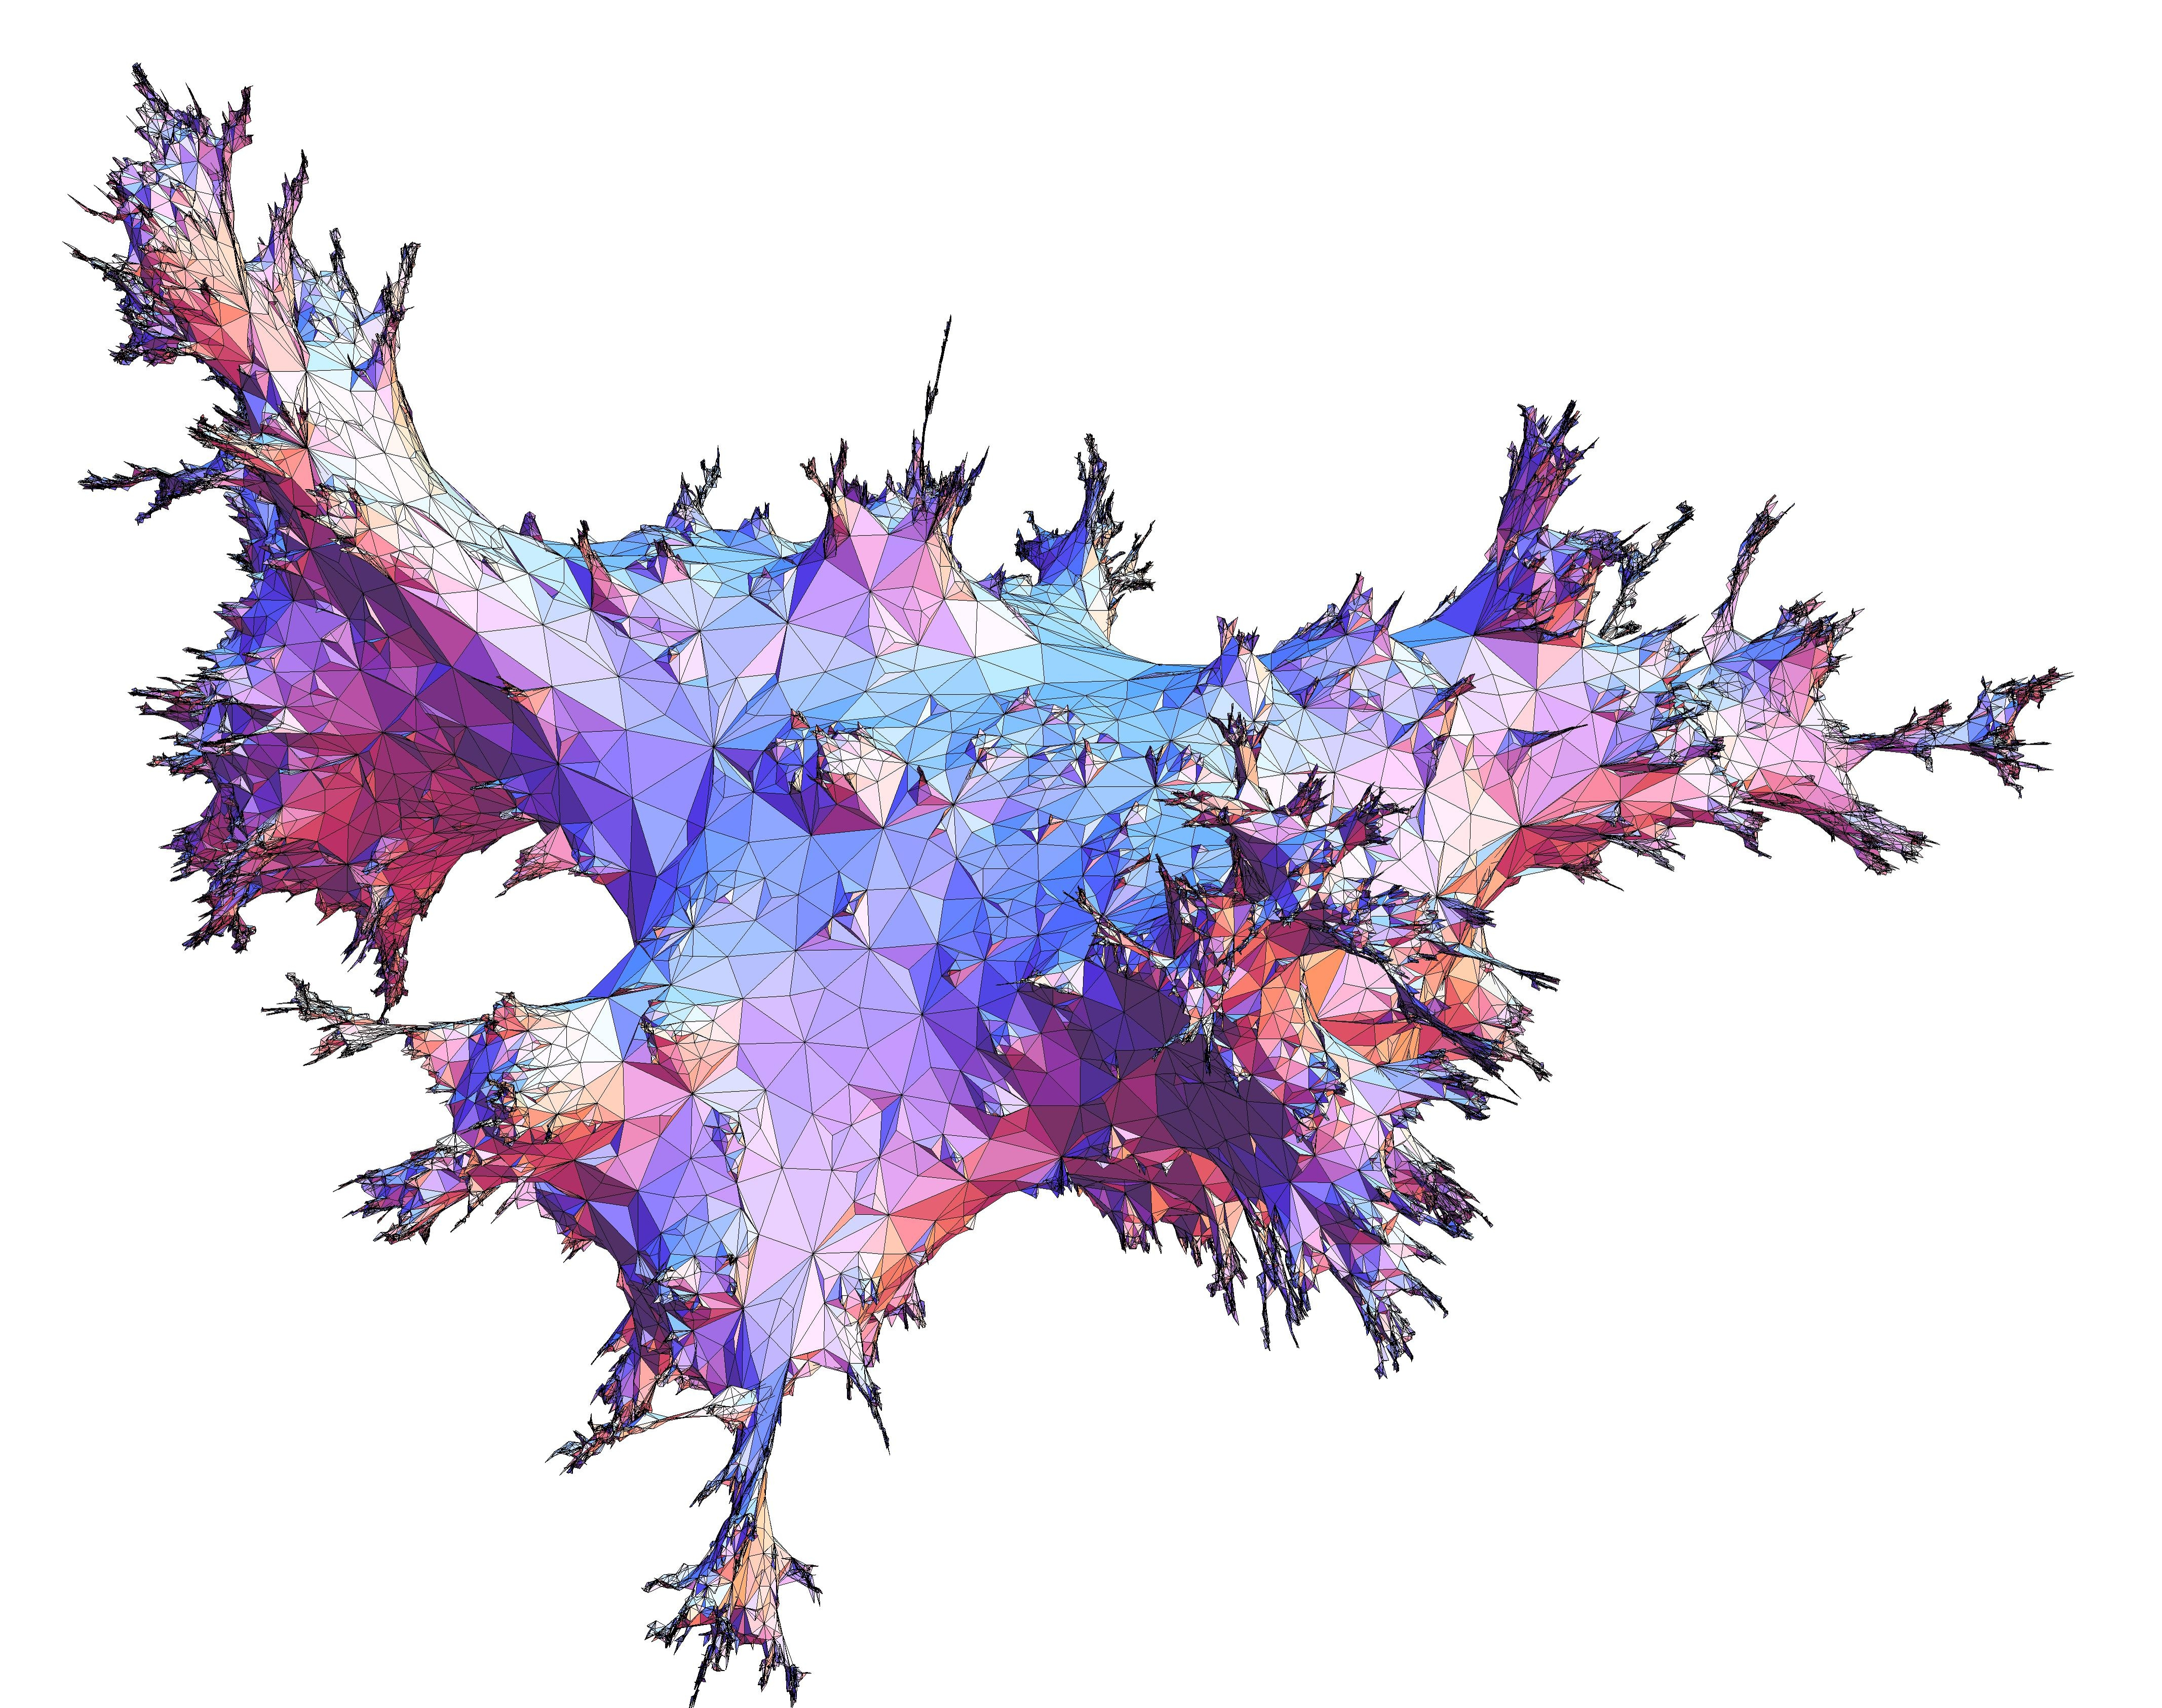
\includegraphics[scale=0.03]{Brownian map.png}
\end{abstract}

\maketitle
\tableofcontents
\section{Measure Theory and Stochastic Process}
Measure Theory is the foundation of modern probability theory. Real analysis is based on the Lebesgue measure derived from outer measure $m_e(E)$. Lebesgue also defined the inner measure $m_i(E)$, and the measurable sets are the ones with $m_e(E) = m_i (E)$. In the more abstract topological space, Caratheodory, Radon and Hausdorff studied more general measures. The note will start with the 'outer measure' point of view, and then move to Caratheodory's view. We will construct a rigorous probability space and introduce the linear operator of expectation $\mb{E}[\cdot]$, and finally, the probability space for stochastic process.



\subsection{Measures in abstract space} More general than the Lebesgue measure $\lambda(\cdot)$ in the real line, we consider a measure on space $(\Omega, \mc{F})$. Before we introduce measures and measurability, we first look into some collection of subsets on $X$.\\

\begin{definition}[p-system]
    Let $\mc{P}$ be a family of sets on $X$, $\mc{P}$ is called a p-system (or a $\pi$-system) if it is closed under intersection, i.e. $$A,B\in \mc{P} \Rightarrow A\cap B \in \mc{P}.$$
\end{definition}
\begin{definition}[semi-ring]
    Let $\mc{R}$ be a family of sets on $X$, $\mc{R}$ is called a semi-ring if for any $A,B\in \mc{R}$ and $A \subset B$, the relative complement $B \backslash$ A can be decomposed into the union of finte disjoint sets in $\mc{R}$. That is, $$\exists C_k \in \mc{R}, k =1,\cdots,n \quad\text{s.t.}\quad B\backslash A = \bigcup_{i=1}^n C_i$$
\end{definition}

\begin{definition}[d-system]
    A collection of sets $\mc{D}$ on $X$ is called a d-system (or $\lambda$-system) if if satisfies:\begin{enumerate}
        \item $X \in \mc{D}$;
        \item $A,B \in \mc{D} $ and $A\subset B$, then $B\backslash A \in \mc{D}$;
        \item For a monotonic sequence $A_n \in \mc{D}$, the limit $A_n \uparrow \cup_{i=1}^\infty A_i \in \mc{D}$
    \end{enumerate}
\end{definition}

\begin{definition}[$\sigma$-field]
    A collection of sets $\mc{F}$ is called a $\sigma$-field on $X$ if it satisfies: \begin{enumerate}
        \item $X\in\mc{F}$;
        \item (closed under complement) $A \in \mc{F} \rightarrow A^c \in \mc{F}$;
        \item (closed under countable union) $A_n \in \mc{F}, \forall n=1,2,\cdots \rightarrow \bigcup_{n=1}^\infty A_n \in \mc{F}$
    \end{enumerate}
    Moreover, given a set $\Omega$, the $\sigma$-field generated by $\Omega$ is defined as the smallest $\sigma$-field that contains $\Omega$, denoted by $\sigma(\Omega)$.
\end{definition}

Next, we can now introduce the famous Dykin's $\pi$-$\lambda$ theorem and its proof. The theorem is useful when the a weaker result would suffice, for instance the measurability of a function, the uniqueness of a measure and so on.\\

\begin{theorem}[$\pi$-$\lambda$ theorem]\label{pilambda}
    Let $\mc{P}$ and $\mc{D}$ be a p-system and a d-system on the same space $X$, if $\mc{P} \subset \mc{D}$ then $\sigma(\mc{P}) \subset \mc{D}$.\\
\end{theorem}

\begin{proof}
    We first claim that a $\mc{F}$ is a $\sigma$-field iff it is a p-system and also a d-system. The necessity is trivial, to prove the sufficiency, the first two property can be verified by $A^c = X \backslash A \in \mc{F}$ by p-system. Lastly, for any countable sequence $(A_n)$, we can construct a montone increasing sequence $(B_n)$ by $B_n := \bigcup_{k=1}^n A_k$ and apply the third property of d-system. Then, we construct a d-system $\mc{D}^*$ that is the smallest d-system that contains $\mc{P}$, if we can show that $\mc{D}^*$ is also a p-system and therefore, a $\sigma$-field, then it implies $\sigma(\mc{P}) \subset \mc{D}^* \subset \mc{D}$. 

    To show $\mc{D}^* $ is indeed a p-system, fix a $B\in \mc{P}$, define a class of set $\mc{E}_1 := \left\{A\in \mc{D}^*: A \cap B \in \mc{D}^*\right\}$. It is easy to show that $\mc{E}_1$ is also a d-system. By construction, $A\in \mc{E}_1 \Rightarrow A\in \mc{D}^*$, that is $\mc{E}_1 \subset \mc{D}^*$. Since $\mc{P} \subset \mc{E}_1$, we have $\mc{D}^* \subset \mc{E}_1 \Rightarrow \mc{D}^* = \mc{E}_1$. 

    Next, for any fixed $B\in \mc{D}^*$, we construct another class of sets $\mc{E}_2 := \left\{A\in \mc{D}^* : A\cap B \in \mc{D}^*\right\}$. Again, one can show that $\mc{E}_2$ is also a d-system. From the above result, $\mc{P} \subset \mc{E}_2$ if $B\in \mc{P}\in \mc{D}^*$, if $B\notin \mc{P}$, $\mc{P} \cap B = \empty \in \mc{D}^* \Rightarrow \mc{P} \subset \mc{E}_2$. Similarly, $\mc{D}^* \subset \mc{E}_2$ and $\mc{E}_2 \subset \mc{D}^* \Rightarrow \mc{D}^* = \mc{E}_2$. 
    
    Now, we have proved that given set $B\in\mc{D}^*$, for any set $A\in \mc{D}^*$ we have $A\cap B \in \mc{D}^*$, thus $\mc{D}^*$ is a p-system. Notice that since $\sigma{\mc{P}}$ is a d-system as well, and by construction $\mc{D}^* \subset \sigma(\mc{P})$. That is, $\sigma(\mc{P}) = \mc{D}^* \subset \mc{D}$.


\end{proof}

\begin{definition}[Measure]
    A set function $\mu: \Omega \rightarrow \mf{R}$  is called a measure on $\Omega$ if it satisfies:
    \begin{enumerate}[(a.)]
        \item $\forall E \in \Omega, \mu(E) \geq 0;$
        \item $\mu(\varnothing ) = 0;$
        \item Countably additive: For any sequence of mutually disjoint subsets $(E_i)_{i\in \mathcal{I}}$ on $\Omega$, where $\mathcal{I}$ can be a countably infinite index set, we have $$\mu\left(\bigcup_{i\in \mathcal{I}}E_i\right) = \sum_{i\in \mathcal{I}}\mu(E_i).$$
    \end{enumerate}
\end{definition}

The next theorem is essential in formulating probability measure. \\
\begin{definition}[pre-measure]
    Let $\mathcal{R}$ be a semi-ring in a give set $X$. A set function $\pi : \mc{R}\rightarrow [0,\infty]$ is called a pre-measure on $(X,\mc{R})$ if it satisfies: \begin{enumerate}
        \item $\pi(\emptyset) = 0$
        \item (finite additivity) If $A_1,A_2,\cdots,A_n \in \mc{R}$ are pairwise disjoint with $\bigcup_{i=1}^n A_i \in \mc{R}$ then $$\pi(\cup_{i=1}^n A_i)=\sum_{i=1}^n \pi(A_i)$$
        \item ($\sigma$-subadditivity) If $A_1,A_2,\cdots,A_n,\cdots \in \mc{R}$ with $A \subset \bigcup_{i=1}^\infty A_i$ then $$\pi(A) \leq \sum_{i=1}^\infty \pi(A_i)$$
    \end{enumerate}
    We say a pre-measure $\pi$ is $\sigma$-finite if there exists a partition $A_1,A_2,\cdots,A_n,\cdots \in \mc{R}$ such that $$\bigcup_{i=1}^\infty A_i = X \quad \text{and} \quad \pi(A_i) <\infty, \forall i =1,2,\cdots$$
\end{definition}

\begin{remark}
    There is an equivalent ways to define pre-measure. A premeasure $\mu_0$ on $\mc{R}$ satisfies \begin{enumerate}
        \item $\mu_0(\emptyset) = 0$
        \item For any sequence of mutually disjoint set $E_1,E_2,\cdots, \in \mc{R}$, and $\cup_{i=1}^\infty E_i \in \mc{R}$ (this condition should be carefully checked since we are dealing with a semi-ring), $$\mu_0\left(\cup_{i=1}^\infty E_i\right) = \sum_{i=1}^\infty \mu_0(E_i).$$
    \end{enumerate}
\end{remark}

\begin{theorem}[Caratheodory's extension theorem]
    Let $\mc{F}_0$ be a semi-ring on a sample space $X$, given a pre-measure $\mu_0$ defined on $\mc{F}_0$, there is a measure $\mu$ such that extends to $\sigma(\mc{F}_0)$. Moreover, if $\mc{F}_0$ is $\sigma$-finite, the extension is unique.\\
\end{theorem}

A proof will be indicated here. The main idea is to construct to so-called outer measure $\mu^*$ in $\mc{F}_0$ and show that the outer measure $\mu^*$ is countably additive on $\sigma(\mc{F}_0)$. We can think of the idea of approximating a postive measurable function by simple function and define the lebesgue integral in the later section.
\begin{proof}
    The first step of the proof is to construct a class of sets that is the finite disjoint union in $\mc{F}_0$, i.e.,
    $$\mc{S} = \left\{A \in X: \exists n, \exists (I_i)_{i=1}^n \in \mc{F}_0 \ \text{are disjoint},\ A= \bigcup_{i=1}^n I_i \right\}.$$

    We can define a measure $\mu_1$ on $\mc{S}$ as following, for any $E\in \mc{S}$,
    $$\mu_1(E) = \sum_{i=1}^n \mu_0(I_i).$$
    To verify that $\mu_1$ is well-defined on $\mc{S}$, that is, the choice of $(I_i)_{i=1}^n$ does not matter, we assume that $E = \bigcup_{k=1}^m J_k$, since $(I_i)_{i=1}^n$ and $(J_k)_{k=1}^m$ are disjoint sequence, we have $$\sum_{i=1}^n \mu_0(I_i) = \mu_0\left(\cup_{i=1}^n I_i\right) = \mu_0\left(\cup_{k=1}^m J_k\right) = \sum_{k=1}^m \mu_0(J_k).$$
    We can consider $\mu_1$ as a middle extension step to construct the measure extension $\mu^*$ on X, note that $\mu_1$ and $\mu_0$ are agree on $\mc{F}_0$. We define the measure $\mu^*$ on $\sigma(\mc{F}_0)$ as following\\

    \begin{definition}[$\mu_0$-outer measure]
        For any set $E\subset X$, the $\mu_0$-outer measure of $E$ is defined by $$\mu^*(E) = \inf \left\{\sum_{i=1}^\infty \mu_0(I_i) : E \subset \bigcup_{i=1}^\infty I_i, (I_i)_{i=1}^\infty \in \mc{F}_0\right\}.$$
    \end{definition}

    It can be easily shown that $\mu^*$ and $\mu_0$ agree on $\mc{F}_0$. However, we need to show that $\mu^*$ obtains the $\sigma$-additivity on $\sigma(\mc{F}_0)$. The nonnegativity is trivial. The next lemma shows that the set function $\mu^*$ has monotonicity and $\sigma$-subadditivity. \\
    
    \begin{lemma}
        The set function $\mu^*$ is monotonic, that is, if $A,B \in \sigma(\mc{F}_0)$ with $A\subset B$ then $\mu^*(A) \leq \mu^*(B)$. Also, $\mu^*$ is $\sigma$-additive, i.e., for any $A_1,A_2,\cdots,\in \sigma(\mc{F}_0)$, we have $$\mu^*(\cup_{n=1}^\infty A_n) \leq \sum_{n=1}^\infty \mu^*(A_n).$$
    \end{lemma}

    To verify the monotonicity of $\mu^*$, notice that any covering $(I_n)_{n=1}^\infty$ of $B$ is also a covering of A, and $\mu^*(A)$ takes the infimum over all coverings. To verify the $\sigma$-additivity, assume that $\mu^*(E_n) < \infty$ (otherwise, it is trivial) and for each $n=1,2,\cdots$, we can find a covering of $E_n$ such that $$\mu^*(E_n) + \frac{\varepsilon}{2^n} \geq \sum_{i=1}^\infty \mu_0(I_{n,i})$$ with $I_{n,1},I_{n,2},\cdots \in \mc{F}_0$. Set $E = \cup_{n=1}^\infty E_n$, then $E \subset \cup_{n=1}^\infty \cup_{i=1}^\infty I_{n,i}$, and $\{I_{n,i}\}_{n\geq 0, i\geq 0}$ is a countable covering of $E$ in $\sigma(\mc{F}_0)$. Hence, 
    $$\mu^*(E) \leq \sum_{n=1}^\infty \sum_{i=1}^\infty \mu_0(I_{n,i}) \leq \sum_{n=1}^\infty \left(\mu^*(E_n) + \frac{\varepsilon}{2^n}\right)= \left(\sum_{n=1}^\infty \mu^*(E_n)\right) + \varepsilon. $$
    As $\varepsilon$ can be arbitarily small, we get $\mu^*(E) \leq \sum_{n=1}^\infty \mu^*(E_n)$ as desired.

    Next, we prove that monotonicity and $\sigma$-subadditivity imply $\sigma$-additivity. \\

    \begin{lemma}
        The set function $\mu^*$ is $\sigma$-additive on $\sigma(\mc{F}_0)$ iff it is both monotonic and $\sigma$-subadditive.  
    \end{lemma}

    The necessity is straightforward. To prove the sufficiency, it is equivalent to verify the $\sigma$-superaddtivity of $\mu^*$. That is, 
    $$\mu^*\left(\bigcup_{n=1}^\infty A_n\right)\geq \sum_{n=1}^\infty \mu^*(A_n).$$
    
    Consider the simplest case $n=2$, recall the alternative of measurable set in real analysis, to show $\mu^*(A \cup B) \geq \mu^*(A) + \mu^*(B)$ is equivalent to show that for any $A,T \in \sigma(\mc{F}_0)$, the following equality holds 
    $$\mu^*(T) \geq \mu^*(T\cap A) + \mu^*(T\cap A^c) ,$$
    as we can take $T = A \cup B$. First consider the simpler case where \underline{$A\in \mc{F}_0$ and $T\in X$}. By definition of $\mu^*$, we can construct a covering $T\subset \cup_{n=1}^\infty I_n$ where $I_1,I_2,\cdots, \in \mc{F}_0$ such that $$\mu^*(T) + \varepsilon \geq \sum_{n=1}^\infty \mu_0(I_n).$$
    For each $n$, as $A\in \mc{F}_0$, $I_n\cap A \in \mc{F}_0$, and $A^c$ is the union of a finite disjoint sets in $\mc{F}_0$ by definition. Therefore $A^c \in \mc{S}$ and $I_n \cap A^c \in \mc{S}$ for each $n$. By the disjoint additivity of pre-measure $\mu_0$ on $\mc{F}_0$, and the construction of $\mu_1$, we have 
    \begin{align*}
        \mu^*(T) + \varepsilon &\geq \sum_{n=1}^\infty \mu_0(I_n)\\
        &\geq \sum_{n=1}^\infty \mu_0(I_n \cap A) + \mu_1(I_n \cap A^c) \\
        &\geq \mu^*(T\cap A) + \mu^*(T\cap A^c).
    \end{align*}
    The las inequality holds since $T\cap A \subset \cup_{n=1}^\infty (I_n \cap A)$ and $T \cap A^c \subset \cup_{n=1}^\infty (I_n \cap A^c)$.

    Next, we complete the proof of the lemma by extending our result in the case that \underline{$A\in \sigma(\mc{F}_0)$}. Let $\mc{D}$ be the collection of sets that super-additivity holds, i.e., $\mc{D}:= \{A\in \sigma(\mc{F}_0): \forall T \subset X, \mu^*(T) \geq  \mu^* ( T\cap A) + \mu^*(T\cap A^c)\}$. We need to show $\sigma(\mc{F}_0) \subset \mc{D}$, note that the semi-ring $\mc{F}_0$ is a p-system and $\sigma(\mc{F}_0) \subset \mc{D}$, we can apply $\pi$-$\lambda$ theorem \ref{pilambda}, it suffices to show that $\mc{D}$ is a d-system. We can verify the three properties of a d-system:
    \begin{enumerate}
        \item $X\subset \mc{D}$ is trivial.
        \item If $A,B\in \mc{D}$ and $B \subset A$, then $A\backslash B \in \mc{D}$ . We have \begin{align*}
            \mu^*(T) &\geq \mu^*(T\cap A) + \mu^*(T\cap A^c) \\
            &\geq \mu^*(T\cap A \cap B) + \mu^*(T\cap A \cap B^c) + \mu^*(T\cap A^c) \\
            &\geq \mu^*(T\cap B) + \mu^*(T\cap B^c \cap A) + \mu^*(T\cap A^c)\\
            &= \mu^*(T\cap B^c \cap A) + \mu^*(T\cap (B\cup A^c)) \\
            &= \mu^*(A\backslash B \cap T) + \mu^*((A\backslash B)^c \cap T)
        \end{align*}
        Therefore $A\backslash B \in \mc{D}$.
        \item If $A_n \in \mc{D}$ is monotonic increasing and $A_n \uparrow A$, then $A\in\mc{D}$. Define a disjoint sequence of sets $(B_n)_{n=1}^\infty$ by letting $B_1 = A_1$, $B_2 = A_2\backslash A_1$,...,$B_n = A_n \backslash A_{n-1} = A_n \backslash \cup_{k=1}^{n-1} A_k$, and $B_n \xrightarrow{n\rightarrow \infty} \cup_{n=1}^\infty A_n$ We have \begin{align*}
            \mu^*(T) &\geq \mu^*(T\cap A_1) + \mu^*(T\cap A_1^c) \\
            &\geq \mu^*(T\cap A_1) + \mu^*(T\cap A_1^c \cap A_2) +\mu^*(T\cap A_1^c \cap A_2^c) \\
            &\ \vdots \\
            &\geq \mu^*(T\cap A_1) + \mu^*(T\cap (A_2\backslash A_1)) + \cdots + \mu^*(T\cap (A_n\backslash A_{n-1})) + \mu^*\left(T\cap \left(\bigcap_{k=1}^n A_k^c\right) \right) \\
            &= \mu^*(T\cap B_1) + \cdots + \mu^*(B_{n}) + \mu^*\left(T\cap \left(\bigcap_{k=1}^n A_k^c\right) \right)\\
            &= \mu^*\left(T\cap \left(\bigcup_{k=1}^n A_k\right)\right) + \mu^*\left(T\cap \left(\bigcup_{k=1}^n A_k\right) ^c\right)
        \end{align*} By monotonicity and $\sigma$-subadditivity of $\mu^*$, we get $$\mu^*(T)\geq \mu^*\left(T\cap \left(\bigcup_{k=1}^\infty A_k\right)\right) + \mu^*\left(T\cap \left(\bigcup_{k=1}^\infty A_k\right) ^c\right).$$ Hence, $\mc{D}$ is a d-system, as required.
    \end{enumerate}

    We've proved the measure $\mu^*$ has both $\sigma$-superaddtivity and $\sigma$-subadditivity on $\sigma(\mc{F}_0)$. We complete the proof of existence. 
    
    We finally complete the proof of the main theorem by showing that the extension is unique. Again, $\pi$-$\lambda$ theorem is applied here. \\

    \begin{lemma}[Uniqueness]
        Suppose that two measures $\mu,\nu$ defined on the same space $(X,\mc{F})$ with $\mu(E) = \nu(E) < \infty$, and there exists a p-system $\mc{P}$ such that $\mu,\nu$ agree on $\mc{P}$ and $\sigma(\mc{P}) = \mc{F}$, then $\mu,\nu$ agree on $\mc{F}$.
    \end{lemma}

    We define the collection of sets $\mc{D} :=\{A\in \mc{F}: \mu({A}) = \nu(A)\}$. We need to show $\mc{F}\subset\mc{D}$, it suffices to show that $\mc{D}$ is a d-system that contains $\mc{P}$. $E \in \mc{D}$ and $\mc{P} \subset \mc{D}$ are trivial. Assume that $A,B \in \mc{D}, B\subset A$, since $\mu(A\backslash B) = \mu(A) - \mu(B) = \nu(A) - \nu(B) = \nu(A\backslash B)$, $A\backslash B \in \mc{D}$. Note that measures are continous with respect to increasing sets. Therefore, $\mu(A_n) \rightarrow \mu(\cup_{n}A_n),\nu(A_n) \rightarrow \nu(\cup_n A_N)$, and since $\mu(A_n) = \nu(A_n)$ for each $n$, $\cup_n A_n \in \mc{D}$. We have proved that $\mc{D}$ is a d-system, and the proof is complete by $\pi$-$\lambda$ theorem.
    \end{proof}

\begin{remark}
    The Caratheodory's extension theorem immediately implies the existence and the uniqueness of lebesgue measure on $(\mb{R},\mc{B}(\mb{R}))$. To see how it is applied, we can take $X = \mb{R}$ and $\mc{F}_0 = \mc{I}$, where $\mc{I}$ is the class of bounded half-open half-closed interval. Recall that the length function $\lambda_0 (I) = |I|$ is well-defined for all $I \in \bar{\mc{I}}$, here $\bar{\mc{I}}$ denotes all bounded and unbounded half-open interval. The pre-measure $\lambda_0$ is $\sigma$-finite since we can let $A_n = (-n,n] $ with $\lambda_0(A_n) = 2n < \infty$ for each $n$.\\
\end{remark}

\begin{corollary}
    Let $S = (0,1]$. We say $F \in \mc{F}_0$ if $F$ can be written as $F = (a_1,b_1] \cup \cdots (a_n,b_n]$. Define $\mu_0(F) = \sum_{n} (b_n - a_n)$. Then $\mu_0$ is a premeasure and there exists an extension of $\mu_0$ on $\sigma(\mc{F}_0)$. 
\end{corollary}
\begin{proof}
    It suffices to verify that $\mu_0$ is countbly-additive over disjoint sets. Let $(F_n)_{n\in \mb{N}}$ be a sequence of disjoint sets and $F = \bigcup_{n=1}^\infty F_n \in \mc{F}_0$. Define the partial union $G_n = \bigcup_{k=1}^n F_k$ and $G_n \rightarrow F$. Define $H_n = F\backslash G_n$, we want to prove that $\mu_0(H_n) \rightarrow 0$. The idea is to prove the contrapositive argument. That is, for the decreasing sequence $(H_n)_{n\in \mb{N}} \in \mc{F}_0$, $\mu_0(H_n) \geq 2\varepsilon,\  \forall n\in \mb{N}\Rightarrow \bigcap_{k} H_k \neq \emptyset$. We choose a sequence of set $J_k \in \mc{F}_0, \bar{J_k} \subset H_k$ such that $\mu_0(H_k \backslash J_k) \geq \frac{\varepsilon}{2^k} $. Since $H_n \backslash \left(\bigcap_{k\leq n} J_k \right) \subset  \bigcup_{k\leq n} \left(H_k \backslash J_k\right)$ by the fact that $(H_n)_{n\in \mb{N}}$ is montonically decreasing. We have \begin{align*}
        \mu_0\left(H_n \backslash \left(\cap_{k\leq n} J_k \right)\right) \leq \mu_0 \left(\cup_{k\leq n} \left(H_k \backslash J_k\right)\right) \leq \sum_{k\leq n} \mu_0\left(H_k \backslash J_k\right) \leq \varepsilon.
    \end{align*}
    Equivalently, \begin{align*}
        2\varepsilon - \mu_0 \left(\cap_{k\leq n} J_k\right) \leq  \mu_0\left(H_n \backslash \left(\cap_{k\leq n} J_k \right) \right)
        \leq \varepsilon
    \end{align*}
    which implies that $\mu_0\left( \cap_{k\leq n} J_k\right) \geq \varepsilon$, that is $\cap_{k\leq n} J_k$ is nonempty for every $n$. 

    To complete the proof, suppose $\cap_{k\in \mb{N}} \bar{J}_k = \emptyset$, then $\{\bar{J}_k^c\}_{k\in \mb{N}} $ is a covering of $[0,1]$. By Hahn-Borel theorem, there is a finite subcover $[0,1] \subset \cup_{k\leq M} \bar{J}_k^c$ which contradicts that $\cap_{k\leq M} J^c \neq \emptyset$.
\end{proof}


\subsection{Random Variable}

We begin with the concept of conditional expectation of a random variable $X$ given a $\sigma-$subalgrebra. We first discuss the case $X \in L^1(P)$ and then further into $X \in L^2$. To begin, we introduce the following theorem.\\

\begin{theorem}[Radon-Nikodym Theorem]
    If $\nu $ is a $\sigma$-finite measures on $\sigma$-finite measure space $(\Omega,\mathcal{F},\mu )$. Then there exists a unique decompostion $\nu = \lambda + \eta$ such that $\lambda \ll \mu, \eta \perp \mu$. Moreover, if $\nu$ is finite then $d\lambda = fd\mu$ for a unique $f\in L^1(\mu)$.
\end{theorem}

\begin{proof}
    There are different ways to prove the result, we introduce a proof via Riesz Representation Theorem. Recall that \\
    \begin{theorem}[Riesz Representation Theorem ]
        Let $f :\mc{H} \rightarrow  \mc{C}$ be a linear functional on a Hilbert Space $\mc{H}$. Then there exists a unique $y \in \mc{H}$ such that $f = fy$.
    \end{theorem}
    We have to prove the existence and uniqueness of $y$. First,
    \begin{proof}
        
    \end{proof}
    
    
    Assume that $\mu,\nu$ are positive and finite. Set $\tau = \mu +\nu$, then $\tau : \Omega \rightarrow \mb{R}$ induces a function space $L^2(\tau)$. Define a linear functional $F$ in $L^2 (\tau)$ ($L^p$ space is a Hilbert space only when $p=2$.) by $F(f) = \int f d\nu$. Notice that 
    \begin{align*}
        \parallel F(f) \parallel  \leq \int |f| d\nu \leq \int |f| d\tau \leq \left(\int |f|^2 d\tau\right)^{\frac{1}{2}} \leq (\tau(\Omega))^\frac{1}{2}
    \end{align*}
    Therefore, $F$ is a bounded linear functional in Hilbert space. There exists a unique $g\in L^2(\tau)$, such that $F(f) = \int fgd\tau$. Moreover, \begin{align*}
        0\leq \nu(E) =\int \mf{1}_E d\nu  = \int \mf{1}_{E} g d\tau = \int_E g d\tau \leq \tau(E)
    \end{align*}
    which implies $g(\Omega) \in [0,1]$. Let $A = \{\omega\in \Omega: g(\omega) = 1\}$, then by the representation,
    $$\int \mf{1}_A d\nu = \int \mf{1} g d\tau = \int \mf{1}_A d\nu + \int \mf{1}_A g d\mu \Rightarrow \mu(A) = 0.$$
    Now we construct the decomposition of $\nu$. Let $\eta (E) = \nu(A\cap E)$ for any $E\in \mc{F}$, then $\eta \perp \mu$, and let $\lambda(E) = \nu(A^c \cap E)$. To verify the absolutely continuity, we observe that for any $n\in \mf{N}$, \begin{align*}
        \int \mf{1}_E (1+g  +\cdots +g^n) d\nu &= \int \mf{1}_E (1+g +\cdots + g^n) gd\nu + \int \mf{1}_E (1)(1+g +\cdots + g^n) gd\mu \\
        \Rightarrow \quad \int_E (1-g^{n+1}) d\nu &= \int_E (1+g +\cdots + g^n) gd\mu
    \end{align*}
    Take $n\rightarrow \infty$, let $h = \lim_{n\rightarrow \infty} (1+g +\cdots + g^n) g$. Then, by monotone convergence theorem, 
    $\lambda(E) = \nu(E) = \int_E d\nu = \int_E hd\mu$, which implies $\lambda \ll \mu$.


\end{proof}

Under the setting of Lebesgue integration, we have some useful results in the limiting behaviors. \\
\begin{theorem}[Monotone Convergence Theorem]
    Suppose $\{f_n\}_{n\in \mb{N}}$ is an increasing sequence of measurable functions defined on measure space $(\Omega,\mc{F},\mu)$. Then, $\int_\Omega\lim_{n\rightarrow \infty}f_n d\mu = \lim_{n\rightarrow \infty} \int_\Omega f_n d\mu $
\end{theorem}

\begin{proof}
    Define $f := \lim_{n\rightarrow \infty} f_n$
\end{proof}

~\\
\subsubsection{$L^1$ case} 
$\mb{E}|X| < \infty$
~\\
\begin{definition}
    Given are a probability space $(\Omega,\mathcal{F},P)$, a $\sigma-$subalgrebra $\mathcal{G} \subseteq \mathcal{F} $ and a random variable $X \in L^1(P)$. We define the conditional expectation of $X$ given $\mathcal{G}$, denoted by $\mb{E}[X|\mathcal{G}]$, to be any random variable $Y$ that satisfies:
    \begin{enumerate}[(i)]
        \item $Y \in L^1(P)$
        \item $\int_E X dP = \int_E Y dP \quad \forall E \in \mathcal{G}$
    \end{enumerate}
\end{definition}

The next thing to be settled is the existence and uniqueness of conditional expectation $\mb{E}[X|\mathcal{G}]$. The alternative proof can be found in \textit{Durrett,Probability Theory and Examply, 4.1}\\
~\\
\vf{Existence.} Recall the Radon-Nikodym Theorem:


~\\
To prove the existence of $\mb{E}[X|\mathcal{G}]$, take $\upsilon(E) \triangleq \int_E XdP$ for all $E \in \mathcal{G}$. Since $X\in L^1(P)$, one can easily check that the well-defined $\upsilon$ is a measure and $\upsilon \ll P$. Apply Radon-Nikodym Theorem:
$$
\int_E XdP = \upsilon(E) = \int_E \frac{d\upsilon}{dP}dP = \int_E YdP
$$
Then $Y$ is a version of $\mb{E}[X|\mathcal{G}]$. \\
~\\
\vf{Uniqueness.}
Assume that $Y$ and $Y'$ both satisfy (i) and (ii). Let $E = A\cup A^c$ where $A$ has measure zero. Then,
$$
\int_E YdP = \int_E Y'dP \Rightarrow \int_E (Y-Y')dP = \int_{A} (Y-Y')dP + \int_{A^c} (Y-Y')dP = 0
$$
Hence, we have $Y = Y' a.s$\\
~\\
Note that (ii) in the definition is equivalent to the following form(take $E$ to be $\Omega$):
$$
     \int_{\Omega} \mb{E}[X|\mathcal{G}]dP = \int_{\Omega} XdP
$$
Moreover, it is also equivalent to:
$$
\int_{\Omega} \mb{E}[X|\mathcal{G}]\cdot Z dP = \int_{\Omega} X\cdot ZdP
$$
for all random variable $Z \in L^1(\Omega,\mathcal{G},P)$. The form is similar to the orthogonal principle. 
\subsubsection{$L^2$ case}
$\mb{E}|X^2| < \infty$
~\\
We found that the well-defined conditional expectation has the same property as a projection. Actually, we can redefine it in $L^2-$theory. 
~\\
\begin{definition}
    For any real random variable $X\in L^2(\Omega,\mathcal{F},P)$, define $\mb{E}[X|\mathcal{G}]$ to be the projection of $X$ onto the closed subspace $L^2(\Omega,\mathcal{G},P)$.
\end{definition}

\subsection{Stochastic Process}
We now move to stochastic process, the process $\left(X_t\right)_{t\in \mathcal{T}}$ is a collection of random variables $X_t$ defined on the measure space $(E,\mathcal{E})$ for every $t\in \mathcal{T}$. Here, $\mathcal{T}$ can be either discrete or continues. The Kolmogorov extension theorem is useful when showing
such existence of a stochastic process whose finite-dimensional distributions are known.\\

\begin{theorem}[Kolmogorov's extension theorem]\label{Kolmogorov_extension}
    For each $n\in \mb{N}$, let $\mu_n$ be a probability measure on $(\mf{R}^n,\mc{B}(\mf{R}^n))$. Assume that $\mu_1,\cdots,\mu_n$ are consistent in the sense that 
    $$\mu_{n+k}(A \times \mf{R}^k) = \mu_n(A),\quad \forall A \subset \mf{R}^n$$
    for any $n\in\mb{N}$. Then there exists a unique probability measure $\mu$ on the product $\sigma$-algebra $\mf{R}^{\infty}$ satisfying 
    $$\mu(A\times \mf{R}^{k}) = \mu_n(A)$$
    for any $n,k$ and any Borel set $A \subset \mf{R}^{n}$
\end{theorem}

We introduce two proofs of the theorem. The first one follows a result in topological space and analysis. \\

\begin{lemma}
    Consider a complete metric space $(X,d)$, and a decreasing sequence of compact sets $F_1 \supset F_2 \supset \cdots \supset F_n \supset F_{n+1} \supset \cdots$. Then 
    $$\bigcap _{i=1}^\infty F_i \neq \emptyset.$$
\end{lemma}

\begin{proof}
    Prove by contradiction. Suppose otherwise $\bigcap_{i=1}^\infty F_i = \emptyset$, then $\bigcup_{i=1}^\infty F_i^c = X$. Since $F_1^c \subset F_2^c \subset \cdots$, and $\forall p\in F_1, p \in F_k^c $ for some $k\geq 2$. Then, $F_2^c,F_3^c\cdots$ form an open cover of $F_1$, by the compactness of $F_1$, there is a finte subcover of $F_1$. That is, $F_1 \subset F_m^c$ for some $m$, which contradicts that $F_1 \supset F_m$.
\end{proof}

\begin{lemma}
    Suppose that we have a collection of non-empty compact set $\{C_n \subset \mf{R}^n: n \geq 1\}$, that satisfies the following condition: if $(x_1,x_2,\cdots,x_{n+1}) \in C_{n+1}$ then $(x_1,\cdots,x_n)\in C_n$ for any positive $n \geq 1$. Then there exists a $(x_1,x_2,\cdots,x_n,\cdots) \in \mf{R}^\infty$ such that $(x_1,x_2,\cdots,x_k) \in C_k$ for any $k\geq 1$.
\end{lemma}

\begin{proof}
    We apply the above lemma to prove the result.
\end{proof}

The second proof follows from Caratheodory's extension theory. 
\begin{proof}
    To construct the desired probability space, we define $\Omega = \mb{R}^{\mc{I}} = \{f: \mc{I} \rightarrow \mb{R}\}$ and cylinder \underline{$\mc{C}_{i_1,i_2,\cdots,i_n}(A_1\times A_2\times \cdots A_n) = \{f \in \Omega : f(i_1) \in A_1,\cdots, f(i_n) \in A_n\}$}. Notice that the collection of cylinders forms a semi-ring. We also define the product topoly on $\Omega$, i.e., $\mc{C}$ is said to be open if $A_1,\cdots,A_n\in\mc{B}(\mb{R})$ are open. 

    The main idea is to define a set function $\mu$ on cylinders and later extend it by Caratheodory's extension theorem. Define $$\mu\left(\mc{C}_{i_1,\cdots,i_n}(A_1,\cdots, A_n)\right) = \mu_{i_1,\cdots,i_n}(A_1\times \cdots\times A_n).$$  If $\mu$ is a premeasure defined on cylinders, we can use Caratheodory's extension theorem to extend $\mu$ to $\sigma$-algebra generated by $\mc{C}$(semi-ring). It suffices to prove that $\mu$ is indeed a pre-measure on cylinders, that is, it is countably additivitive over finite disjoint sets. (Note that the consitency condition is used in defining $\mu$.)

    Assume that $U_1,U_2,\cdots$ are disjoint cylinders and let $V =\bigcup_{n\in \mb{N}} U_n$. We want to show : $\mu(V) = \sum_{n\in \mb{N}} \mu(U_n)$. Consider partial sums: $$\mu(V) \geq \mu\left(\bigcup_{n=1}^N U_n\right) = \sum_{n=1}^N \mu(U_n), \ \forall N \Rightarrow \mu(V) \geq \sum_{n=1}^\infty \mu(U_n).$$

    To prove the reverse direction, we use the property of compactness. Since $V$ is also a cylinder, let $V = \mc{C}_{i_1,\cdots,i_n}(A_1\times \cdots \times A_n)$. Choose $\tilde{A} \subset A_1\times \cdots\times A_n\in \mb{R}^n$  such that $\tilde{A}$ is compact and $$\mu(\tilde{A}) + \varepsilon \geq \mu_{i_1,\cdots,i_n}(A_1\times \cdots \times A_n)$$, where $\mu_{i_1,\cdots,i_n}$ is given by assumption. 

    Similarly, let $U_j = \mc{C}_{{i_1^j},\cdots,i^j_{n_j}}(B^j_1\times \cdots \times B^j_{n_j})$ for each $j\in \mb{N}$. We choose an open set $\tilde{B}_j \in \mb{R}^{n_j}$ for each $j$ such that  $B^j_1\times \cdots \times B^j_{n_j} \subset \tilde{B}_j $ and $$\mu(U_j) = \mu_{i^j_1,\cdots,i^j_{n_j}}(B_1^j \times \cdots \times B_{n_j}^j) \geq \mu_{i^j_1,\cdots,i^j_{n_j}}(\tilde{B}_j) - \frac{\varepsilon}{2^j}.$$

    Recall that $V = \mc{C}_{i_1,\cdots,i_n} (A_1\times \cdots \times A_n) = \bigcup_{n=1}^\infty U_n = \bigcup_{j=1}^\infty \mc{C}_{i^j_1,\cdots,i^j_{n_j}}(B^j_1\times \cdots \times B^f_{n_j})$, by construction, we have $\tilde{A} \subset \bigcup_{j=1}^\infty \tilde{B}_j$. Since $\tilde{A}$ is compact, there exists a finite subcover $\bigcup_{j=1}^F \tilde{B}_j \supset \tilde{A}$. Therefore, $$\mu(V) - \varepsilon \leq \mu(\mc{C}_{i_1,\cdots,i_n}(\tilde{A})) \leq \sum_{j=1}^F \mu (\mc{C}_{i^j_1,\cdots,i^j_{n_j}}(\tilde{B}_j)) \leq \sum_{j=1}^\infty \mu (\mc{C}_{i^j_1,\cdots,i^j_{n_j}}(\tilde{B}_j)) \leq \sum_{j=1}^\infty \left[\mu(U_j) + \frac{\varepsilon}{2^j}\right],$$ or equivalently $\mu(V)  \leq \sum_{j=1}^\infty \mu(U_j) + 2\varepsilon$. The reverse direction is verified and $\mu$ is countably additive over disjoint sets. 
\end{proof}

\subsection{Martingale}
Based on the conditional expectation, we can formally define martingales in language of measure theory. We first look at the discrete case.
~\\
\begin{definition}[Filtration]
    The filtration is defined as a sequence of increasing $\sigma-$subalgrebra
    $$ (\mathcal{F}_n)_{n \ge 0} \triangleq \mathcal{F}_0 \subseteq \mathcal{F}_1 \subseteq \mathcal{F}_2 \subseteq \cdots$$ and 
    a sequence of random variable $(X_n)_{n \ge 0}$ is \xt{adapted} to the filtration $(\mathcal{F}_t)_{t \ge 0}$ if $X_n$ is $\mathcal{F}_n-$measurable for all $n$.
\end{definition}
~\\
\begin{definition}[Martingale]
    If $(X_n)_{n \ge 0}$ is a sequence of random variables satisfy:
    \begin{enumerate}[(i)]
        \item $X_n \in L^1(P)$, i.e. $\mb{E}[|X|] < \infty$
        \item $(X_n)_{n \ge 0}$ is adapted to $(\mathcal{F}_n)_{n\ge 0}$
        \item $\mb{E}[X_{n+1}|\mathcal{F}_n] = X_n  \quad \forall n$
    \end{enumerate}
    then $X$ is said to be a martingale w.r.t $\mathcal{F}_n$
\end{definition}
Martingales are used to model fair game. The common applications include gamble's ruin. 
~\\
\begin{definition}[Stopping Time]
    A nonnegative random variable $T:\Omega \rightarrow {0,1,\cdots,\infty}$ is a stopping time if
    $$\{T=n\} = \{\omega\in\Omega|T(\omega) = n\} = T^{-1}(n) \in \mathcal{F}_n$$
    
\end{definition}
~\\
\begin{theorem}[Doob's optional stopping theorem]
If $(X_n)_{n\ge 0}$ is a martingale adapted to the filtration $(\mathcal{F}_n)_{n\ge 0}$ and $T$ is the corresponding stopping time,
and at least one of the following holds:
% \begin{enumerate}[(a.)] 
%     \item $\exists n \in \mathbb{N}, s.t. P(T \le n) = 1$
%     \item $
% \end{enumerate}

    
\end{theorem}

\newpage
\section{Markov Process and Ergodic Theory}

\subsection{Markovian process} We then recall the Markov property, which refers to the memoryless property of a stochastic process. It means that the current state is a sufficient statistic of the future states.
~\\
\begin{definition}[Markov Property]
    Suppose $(X_t),t\in T \subset \mathbb{R}$.For any set of times $t_1 < t_2<\cdots <t_n$ and any borel set $B$
    $$ P(X_{t_{n+1}}\in B | X_{t_n}, X_{t_{n-1}},\cdots,X_{t_1}) = P(X_{t_{n+1}}\in B | X_{t_n})$$
\end{definition} 

The difference between markov property and martingale is that:
\begin{itemize}
    \item Markov property requires the entire distribution of $X_{t+s}$ depends on the past only through $X_s$
    \item In a maringale, the expectation of $X_{t+s}$ depends on the past only through $X_t$ with filtration.
\end{itemize}
Markov process can be well-defined as follows:
~\\
\begin{definition}[Markov Process]
    Let $(\Omega,\mathcal{F},P)$ be a probability space. The stochastic process $\mathbb{X} = \{X_n; n \geq 1\}$ is said to be Markovian if $$\mathbb{E}$$
\end{definition}
~\\

We can extend the Markov property to random times. Consider the random shift operator 

\begin{definition}[Strong Markov Property]

\end{definition}

\newpage
\section{Brownian motion}
In this section, we will introduce the well-known example of a continous time stochastic process--- Brownian Motion and the general Levy process as well.
\subsection{Constructions of BM} 
BM can be considered as the limiting random walk model with scaling the stepsize and time. The formal definition is the following:
~\\
\begin{definition}[Brownian Motion]
    A stochastic process $(B_t)_{t\ge 0}$is called a brownian motion if
    \begin{enumerate}[(i)]
        \item $B_0 = 0\ \ a.s$
        \item $(B_t)_{t\ge 0}$ has independent increments. i.e $(B_{t_j} - B_{t_i}) \perp\!\!\!\perp (B_{t_n} - B_{t_m}) , i < j, m<n$. 
        \item $(B_t)_{t\ge 0}$ has stationary normal increments. i.e. $(B_t - B_s) \sim \mathcal{N}(0,t-s)$
        \item $t\mapsto B_t(\omega)$ is continuous almost surely.
    \end{enumerate} 
\end{definition}

There are some variation of Brownian Motion, such as d-dimensional BM with drift, (standard) complex BM. Furthermore, we can extend the sense of 'random measure' of a path into a plane and construct a so-called \textbf{Gaussian Free Field}. \\


\subsubsection{Construction and existence of BM}
We note that the proof of the existence of a standard Brownian motion, and the almost surely continuity of $t\rightarrow B_t(\omega)$ are nontrivial. We refer to Chapter 2 in \cite{113} for the constructions and the proofs. There are three approaches to fix the issue:
\begin{itemize}
    \item We approximate Brownian motion by 1-d random walk, or more specifically,
    \item We apply Donsker's invariance principle of functional CLT and Prokhov's criterion to prove the convergence. 
    \item Consider Ito's isometry (will be discussed later), we can either use fourier basis (Wiener's construction) or Haar basis (Levy-Ciesielski's construction) construct Brownian motion as a random vector.
\end{itemize}

Additionally, we can use Kolmogorov's extension theorem \ref{Kolmogorov_extension} to construct Brownian motion by its density. Note that the family of function given by $$f_{B_{t_1,}\cdots,B_{t_n}} (x_1,\cdots,x_n) = \frac{1}{(2\pi)^{\frac{n}{2}}}\prod_{j=1}^n \frac{1}{\sqrt{t_j - t_{j-1}}} \exp \left(-\frac{1}{2} \frac{(x_j - x_{j-1})^2}{t_j - t_{j-1}}\right)$$ satisfies Kolmogorov's consistency condition. For the almost surely continuity, we refer to Kolmogorov's countinuity theorem below. 

Note that we are dealing with orthonomal basis in Hilbert space $L^2([0,1])$. Orthonormal bases in a Hilbert Space are useful because they allow one to approximate any function in the Hilbert Space with a linear combination of the basis elements, thus we can construct BM to be the linear combination of basis. A little reminder of fourier analysis, every function $f\in L^2([0,1])$ can be represented as $$f(x) = \sum_{n=1}^\infty \left(\int_0^1 f(t)e^{-in2\pi t} dt\right)e^{in2\pi t}$$. We can state the next useful lemma:\\

\begin{lemma}
    Let $\mc{H} = L^2(\Omega)$ be a centered Gaussian space. $\{g_n\}_{n\in \mb{N}}$ is the orthonormal basis in $\mc{H}$. If $\{f_n\}_{n\in \mb{N}}$ is an orthonormal basis in $L^2([0,1])$, then $\{g_k f_n\}_{n,k\in \mb{N}}$ forms an orthonormal basis in $L^2(\Omega \times [0,1])$
\end{lemma}


For the (iv.) property that states BM has almost surely continuous sample path, we introduce Kolmogorov's continuity theorem and the primitive idea of chaining arguement. \\

\begin{theorem}[Levy's construction]
    
\end{theorem}

\begin{theorem}[Kolmogorov's continuity theorem]
    Let $\{X(t)\}_{t\in [0,T]}$ be a real-valued random process defined on $(\Omega,\mc{F})$ for each $t$, such that $\exists \alpha ,\beta > 0, \beta \leq \alpha,$ $\forall t,s \in [0,T]$, we have $$\mb{E}\left|X(t) - X(s)\right|^\alpha \leq C|t-s|^{1+\beta}.$$ Here $C$ is a constant indepent of $\alpha,\beta$. Then, $\{X(t)\}_{t\in [0,T]}$ has a modification $\{Y(t)\}_{t\in [0,T]}$ such that $Y\in \text{Lip}_{\gamma}([0,T])$ for any $0< \gamma < \frac{\beta}{\alpha}$.
\end{theorem}

\begin{proof}
    WLOG, we set $T=1$. Let $\Delta_k = \left\{\frac{j}{2^k}, j = 0,1,\cdots,[2^k]\right\}$ and $\Delta = \bigcup_k \Delta_k$. Note that $\Delta$ is a dense set in $[0,1]$. Let $\gamma < \frac{\beta}{\alpha}$ For any $s,t\in [0,1]$, by Markov's inequality,  \begin{align*}
        \mb{P}\left(|X(t) - X(s)|^\alpha \geq |t-s|^{\gamma\alpha} \right) &\leq \frac{\mb{E}\left(|X(t) - X(s)|^\alpha\right)}{|t-s|^{\alpha \gamma}} \\
        &\leq C|t-s|^{1+\beta - \alpha\gamma} =: C|t-s|^{1+\theta}
    \end{align*}
    Therefore, we have \begin{align*}
        \sum_{k\in\mb{N}} \sum_{j=0}^{[2^k]-1} \mb{P}\left(\left|X\left(\frac{j+1}{2^k}\right) - X\left(\frac{j}{2^k}\right)\right| > 2^{-k\gamma}\right) &\leq \sum_{k\in \mb{N}} \sum_{j=0}^{[2^k]-1} C(2^{-k})^{1+\theta} \\
        &\leq C\sum_{k\in \mb{N}} 2^{-k\theta} <+\infty
    \end{align*}
    By Borel-Cantelli lemma, there exists $\Omega_0 \in \mc{F}$ , $\mb{P}\left(\Omega_0^c\right) = 0$ such that for any fixed $\omega \in \Omega_0$, $\exists k_0(\omega) \in \mb{N}$, whenever  $k\geq k_0$, for all $j = 1,\cdots,[2^{k_0}-1]$, we have $$\left|X_\omega\left(\frac{j+1}{2^k}\right) - X\left(\frac{j}{2^k}\right)\right| \leq 2^{-k\gamma}.$$
    Next, let $k,n > k_0(\omega)$, we will find a constant $C_{n,k} > 0$ such that $\forall s,t \in \Delta_n$ , if $|t-s|< 2^{-k}$, then $|X(t)-X(s)| \leq C_{n,k}$. Observe that when $n>k$, $C_{n,k}$ is not nontrivial. Here, $C_{n,k}$ will be defined recursively as the following:

    Assume that $t,s \in \Delta_{n+1} \supset \Delta_n $, and $|t-s| \leq 2^{-k}$. Then, we choose $t',s' \in \Delta_n$ such that $t\leq t' \leq s' \leq s$ and $|t-t'|, |s-s'| \leq 2^{-(n+1)}$. By triangular inequality, \begin{align*}
        |X(t) - X(s)| &\leq |X(t) - X(t') | + |X(t') - X(s')| + |X(s') - X(s)| \\
        &\leq 2\cdot 2^{-(n+1)\gamma} + C_{n,k} =: C_{n+1,k}
    \end{align*}
    By the inductive construction of $C_{n,k}$, note that for any $n > k_0(\omega)$, $C_{n,k} = \sum_{n\geq k} 2\cdot 2^{-(n+1)\gamma} \leq \bar{C} \cdot 2^{-k\gamma}$ (sum over $n$). Therefore, $\forall s,t \in \Delta, \forall k > k_0(\omega)$, whenever $|t-s| \leq 2^{-k} \Rightarrow |X(t) - X(s)| \leq \bar{C} \cdot 2^{-k\gamma}$. Finally, take any $t\neq s, t,s\in \Delta$. Assume that $|t-s| < 2^{-k_0}$ (we are now verifying holder continuity), and choose $k > k_0$ where $2^{-(k+1)} \leq |t-s| \leq 2^{-k}$. That is, \begin{align*}
        |X(t) -X(s)| \leq \tilde{C}_k \cdot |t-s|^\gamma.
    \end{align*}
    To complete the proof, let $\omega \in \Omega_0, t\in [0,1]$. Define $Y(t) = \lim_{n\rightarrow \infty} X(t_n)$ where $\{t_n\}_{n\in \mb{N}} \subset \Delta$ is any sequence such that $t_n \rightarrow t $ as $\Delta$ is dense in $[0,1]$  For $\omega \in \Omega_0^c$ ,set $Y(t) = 0$. Then $X(t_n) \xrightarrow{\mb{P}} X(t)$  and $X(t)$ is holder continuous by the fact that holder space is Banach, and $Y(t) = X(t)\  a.s.$
\end{proof}

\subsubsection{Characterizations of BM}

Observe that a standard BM is a martingale with respect to itself. To show this, it is sufficient to verify (iii) in the definition 1.2.2, for any $ 0 \le s <t$:
\begin{align*}
    \mb{E}[B_{t+1}|B_t] &= \mb{E}[B_{t+1}-B_t +B_t | B_t] \\
    & = \mb{E}[B_{t+1}-B_t|B_t-B_0] + \mb{E}[B_t|B_t]\\
    & = \mb{E}[B_{t+1}-B_t] + B_t \\
    & = 0 + B_t = B_t
\end{align*}
Then we consider the martingale w.r.t $(B_t)_{t\ge 0}$ which is also a transformation of $(B_t)_{t\ge 0}$. Let


~\\
The theorem that connects BM to martingale theory is Levy's characterization of Brownian Motion:\\
\begin{theorem}[Levy's Theorem]
    Let $(X_t)_{t\ge 0}$ be a continuous process adapted to the filtration $(\mathcal{F}_t)_{t\ge 0}$. $(X_t)_{t\ge 0}$ take the value in $\mathbb{R}$, if it satisfies:
    \begin{enumerate}[(i)]
        \item $M_t \triangleq X_t - X_0$ is a local martingale w.r.t $\{\mathcal{F}_n\}$
        \item $(M_t^2 -t)_{t\ge 0}$ is also a local martingale.
    \end{enumerate}
    Then, $(X_t)_{t\ge 0}$ is a Brownian Motion.
\end{theorem}

Levy's theorem characterized standard Brownian Motion by deriving two maringales. Moreover, the characterization of the standard Brownian Motion can be extended by exactly one continuous-time martingale. \\


\subsection{Modulus of continuity}

In this section, we will discuss more about the smoothness of Brownian motion path. The famous theorem of the modulus of continuity is the following:\\
\begin{theorem}[Levy's continuity theorem]
    For any $T>0$,
   $$\lim_{h\rightarrow 0} \sup_{t\in [0,T-h]} \frac{ |B(t+h) - B(t)|}{\sqrt{2h\log \frac{1}{h}}} = 1 \quad a.s.$$
\end{theorem}

\begin{proof}
    Let $n\in \mb{N}$, set $t_j = j\cdot e^{-n}$, $j = 1,\cdots,[e^n]$. Then, by tail probability estimation, \begin{align*}
        \mb{P}\left(|B(t_{j+1}) - B(t_j)| > \alpha \sqrt{2 e^{-n}\cdot n}\right) &= \mb{P}\left(|Z| > \alpha \sqrt{2n}\right) \\
        &\geq \frac{C}{\alpha\sqrt{2n}} \exp\left(-\frac{\alpha^2 \cdot 2n}{2}\right) \\
        &\geq \exp\left(-(\alpha^2 + \varepsilon) n\right).\\
    \end{align*}
    This implies \begin{align*}
        \mb{P}\left(\left|B(t_{j+1}) - B(t_j)\right| \leq \alpha \sqrt{2e^{-n}\cdot n},\ \forall j=1,\cdots,[e^n]\right) &\leq  \Pi_{j=1}^{[e^n]} \left(1- \exp(-(-\alpha^2 + \varepsilon)n)\right) \\
        &\leq \exp\left(\exp\left(-(\alpha^2 + \varepsilon) \cdot n\right)e^n\right) \\
        &=\exp\left(\exp\left(-(\alpha^2 + \varepsilon -1) \cdot n\right)\right).
    \end{align*}
    We can take some $\varepsilon > 0$ such that $\alpha^2 + \varepsilon > 1$. Therefore, when $n\uparrow \infty$, the joint probability is approximately $o(1)$. 

    Next, recall the levy's construction of Brownian Motion, $B(t) = \sum_{n=0}^\infty \sum_{k=1 }^{[2^n]} g_{n,k} f_{n,k}$, where $\{g_{n,k}\} \sim \mc{N}(0,1)$ i.i.d. and $\{f_{n,k}\}$ is the haar basis of $L^2([0,1])$.

    We use union bound to show that for each $n$, 
    \begin{align*}
        \mb{P}\left(\max_{k\in [2^n]} g_{n,k} \geq C\right)
    \end{align*}
\end{proof}

\begin{theorem}[Paley-Wiener-Zygmund]
 Brownian Motion $B(t)_{t\in [0,+\infty]}$ is nowhere differentiable $a.s.$
\end{theorem}

\begin{proof}
    
\end{proof}


\subsection{Strong Markov Property of Brownian Motion}
For the discussion of Markov property, let $\mc{F}(t)$ be the natural filtration of $B(t)$ and define $$\mc{F}^+_{t_0} = \bigcap_{t > t_0 }\mc{F}_t.$$

Note that the filtration $\{\mc{F}^+_t\}$ is larger than natural filtration and it is right-continuous. \\

\begin{lemma}
    For any $t_0 > $, the process $\{B(t+t_0) - B(t_0)\}_{t\in [0,+\infty]}$ is a standard BM indepent of $\mc{F}_{t_0}$. 
\end{lemma}

\begin{proof}
    We prove the lemma by using the scheme of Kolmogorov extension theorem. Let $A \in \mc{F}_{t_0},C\in \mc{C}([0,+\infty])$ be measurable sets, we have to check that $$\mb{P}(B(t+ t_0 ) - B(t_0)\in (C\cap A)) = \mb{P}(\bar{B}(t) \in C) + \mb{P} (\bar{B}(t) \in A) \quad \quad (*)$$

    where we denote $\bar{B} (t) = B(t+t_0) - B(t_0). $ Consider the marginals, let $0 \leq s_1 \leq \cdots \leq s_k \leq t_0, t_0 \leq t_1 \leq \cdots \leq t_m$ and define the cylinders $$A = \mc{C}_{s_1,\cdots, s_k}(\tilde{A}),\quad C = \mc{C}_{t_1 - t_0,\cdots, t_m -t_0}(\tilde{C})$$
    where $\tilde{A} \in \mc{B}(\mb{R}^k), \tilde{C} \in \mc{B}(\mb{R}^m)$. Then $(*)$ holds and we ca pass the limit of cylinders to general sets.
\end{proof}

Let $\bar{B}(t)$ be defined in the last lemma, we have the following result. \\
\begin{lemma}
    For some fixed $t_0\in [0,+\infty)$, $(\bar{B}(t))_{t\in [0,+\infty)}$ is a Brownian motion independent of $\mc{F}_{t_0}^+$. 
\end{lemma}

\begin{proof}
    
\end{proof}

\subsection{Brownian Motion and Random Fractals}
In this section we will briefly discuss some geometrical properties of some particular random sets, e.g. zero set $\mathcal{Z}_0 := \{t\in [0,1]: B_t = 0\}$. We will introduce some dimension index to measure the random sets, namely, Hausdorff dimension, packing dimension and Minkowski dimensions. This section is a brief literature review of the progress in singularities. 

Levy's modulus of continuity is a famous result in measuring the unsmoothness of the sample path of BM. \\

The famous work by Orey and Taylor \cite{Orey&Taylor} has proved that the Hausdorff dimension of $\lambda$-fast point 
$$E(\alpha) = \left\{t\in [0,1] : \lim \sup_{h\rightarrow 0} \frac{B(t+h) - B(t)}{\sqrt{2h\log \frac{1}{h}}} \geq \alpha\right\}$$

is $\text{dim}_{H} E(\alpha) = 1-\alpha^2$ with probability 1.


\subsection{Levy Process}
A Levy process is an adapted stochastic process with independent and stationary increments. Brownian Motion is an example of Levy process with normally distributed stationary and independent increments. Other examples includes Poisson process.

An very important feature of Levy process is its infinite divisibility. The infinite divisibility of a random variable means the following\\
\begin{definition}[Infinite divisibility]
    A random variable $X$ is called infinitely divisible if, for any $n\in \mb{N}$, there exist i.i.d random variables $\left(X_1^{(n)},X_2^{(n)},\cdots,X_n^{(n)}\right)$ such that, 
    $$X \disteq X_1^{(n)} + X_2^{(n)} +\cdots +X_n^{(n)} $$
\end{definition}

By definition, $X$ is infinitely divisible means that its probability law has $n$-th convolution root, and the characteristic function has $n$-th root.

The next theorem studied the properties of characteristic function of a Levy Process, and provide a representation of Levy process.\\
\begin{theorem}[Levy-Khintchine formula]
    Suppose that the random process $(X_t)_{t\geq 0}$ has the probability law of $\mu$. The characteristic exponent , denoted by $\Psi (\lambda)$, 
    $$\Psi(\lambda) = \int_{\mf{R}} e^{i\lambda x}\mu(dx)$$
    exists for all $t$,
    then $(X_t)_{t\geq 0}$ is a Levy process if and only if there exists a triple $(a,\sigma,\Pi)$, such that $\Psi(\lambda)$ satisfies
    $$\Psi(\lambda) = i\langle a,\lambda\rangle + \frac{1}{2}\sigma^2\lambda^2 + \int_{\mf{R}} (1-e^{i\langle \lambda, x \rangle} + i\langle \lambda,x \rangle \mf{1}_{|x|<1}) \Pi(dx) $$
    where $a \in \mf{R}, \sigma \geq 0$ and $\Pi$ is a measure supported on $\mf{R}\setminus\{0\}$ that satisfies $\int_{\mf{R}} (1\wedge x^2)\Pi(dx) < \infty$.
\end{theorem}

\newpage
\section{Limit Theorems}
Motivated by Kolmogorov-Smirnov test, which states a result of empirical distribution convergences to Brownian bridge, I am interested in the extended definition of convergence. The chapter follows the book \textit{Limit Theorems for Stochastic Process} by Jean Jacod and Albert N. Shiryaev, 2002. \\
~\\
We will introduce some famous results in real analysis and functional analysis, which is useful to establish some limit theorems. This part refers to the lecture note \textit{C8.6 Limit Theorems and Large Deviations in Probability} by Professor Qian.\\

\begin{theorem}[Ascoli-Arzelà's Lemma]
    A family of functions $\mc{F} \subset \mc{C}(X,\mb{R}^d)$, where $(X,d)$ denotes a compact metric space, is relatively compact if and only if:\begin{enumerate}
        \item $\mc{F}$ is uniformly bounded.
        \item $\mc{F}$ is equicontinuous in the sense that $$\lim_{\delta \downarrow 0} \sup_{f\in \mc{F}, d(s,s')< \delta} |f(s) - f(s')| = 0.$$
    \end{enumerate}
\end{theorem}

\begin{proof} We first prove the "if" part:\\
    It is enough to prove that $\mc{F}$ is sequentially compact, i.e. every function sequence $\{f_i\}_{i=1}^\infty \subset \mc{F}$ has a convergent subsequence. Since $(X,d)$ is a compact metric space, and for each $n$, the collection of open balls $X \subset \bigcup_{n=1}^\infty B(x_n,\frac{1}{n})$ is an open cover of $X$, where $\{x_i\}_{i=1}^n \in X$. Then it induced a finite subcover $\{B(x_i,\frac{1}{n})\}_{i=1}^{N}$ and a "$\frac{1}{n}$-dense" set of $X$.  By the Bolzano-Weierstrass theorem, $\{f_{n}(x_1)\}_{n=1}^\infty$ is uniformly bounded implies that there is a convergent sequence $\{f_{1,k}(x_1)\}_{k=1}^\infty$. We construct the subsubsequence $\{f_{2,k}\}_{k=1}^\infty \subset \{f_{1,k}\}_{k=1}^\infty$ such that $\{f_{2,k}(x_2)\}_{k=1}^\infty$ converges at $x_2$. Repeat the process $n$ times and we get the sequence $\{g_n\}_{n=1}^\infty := \{f_{n,n}\}_{n=1}^\infty$. To see that $\{g_n\}_{n=1}^\infty$ is the desired convergent subsequence, let $\epsilon > 0$ be given, by equicontinuity, there is a $\delta > 0$ such that $|g_n(x) - g_n(y)| < \frac{\epsilon}{3}$ whenever $d(x,y) < \delta$ for each $n$. By compactness of $X$, it is possible to find a finite subcover of $X$, fix a number $N$ such that $\{B(x_n,\frac{1}{n})\}_{n=1}^N$ is a finite subcover and at the meantime $N > \frac{1}{\delta}$. In the construction of $\{g_n\}_{n=1}^\infty$, we note that there exists a number $M$ such that $$|g_m(x) - g_n(x)| < \frac{\epsilon}{3} \quad \forall s \in \{x_n\}_{n=1}^N$$
    if $m,n > M$. If $m,n > M$, for an arbitary $x' \in \{x_i\}_{i=1}^N$, we have $d(x,x') < \delta $ and 
    \begin{align*}
        |g_n(x) - g_m(x)| &\leq |g_n(x) - g_n(x')| + |g_n(x') - g_m(x')| + |g_m(x') - g_m(x)| \\
        &\leq \frac{\epsilon}{3} + \frac{\epsilon}{3} + \frac{\epsilon}{3} = \epsilon
    \end{align*}
    That is, the sequence $\{g_n\}_{m=1}^\infty$ is uniformly Cauchy, and thus uniformly convergent.\\

    The other part of the proof: assume that $\mc{F}$ is relatively compact, and thus sequentially compact. Prove by contradiction: suppose otherwise that $\mc{F}$ is not equicontinuous, that is, there exists $\varepsilon_0 > 0$ such that for each $n$, there is at least a function $f\in \mc{F}$, denoted by $f_{(n)}$, and a point $x_{(n)}$ that satisfy $$|f_{(n)}(x_{(n)}) - f_{(n)}(x')| > \varepsilon_0 \quad \text{where} \ d(x_{(n)}, x') < \frac{1}{n}.$$ 
    The sequence of function $\{f_{(n)}\}_{n=1}^\infty$, by the sequentially compactness of $\mc{F}$, has a convergent subsequence $\{f_{(n)_k}\}_{k=1}^\infty$. Assume $f_{(n)_k} \rightarrow f \in \mc{F}$ uniformly, then $f$ is also continuous. We can choose a number $K$ such that whenever $k>K$, $\sup_{x\in X} |f_{(n)_k}(x) - f(x)| < \frac{\varepsilon_0}{3}$ by convergence. However, we have \begin{align*}
        |f(x_{n_k}) - f(x)| &\geq |f_{(n)_k}(x_{n_k}) - f_{(n)_k}(x)| - |f_{(n)_k}(x) - f(x)| - |f(x_{n_k}) - f_{(n)_k}(x_{n_k})| \\
        &\geq \varepsilon_0 - \frac{\varepsilon_0}{3} -\frac{\varepsilon_0}{3} = \frac{\varepsilon_0}{3}
    \end{align*}
    for $d(x_{n_k},x) < \frac{1}{n_k}$, which contradicts the continuity of $f$. Finally, we prove that $\mc{F}$ is uniformly bounded, again, we prove by contradiction, suppose that $\mc{F}$ is unbounded, that is, there exists a $x_0 \in X$ such that for some $f_1(x_0)$ in the space $\mc{F}$, we can find a $f_2(x_0) $ such that $|f_1(x_0),f_2(x_0)| > 1$, moreover, the unboundedness allows us to repeat the procedure infinitely many times. We can find $f_3 \in \mc{F}, \text{where} |f_3(x_0) - f_k(x_0)| > 1 $ for $k =1,2$. Therefore, there is a sequence of functions $\{f_n\}_{n=1}^\infty$ that $|f_m(x_0) - f_n(x_0)| > 1$ for any $n\neq m$. It contradicts with the sequentially compactness as it is impossible to find a Cauchy (convergent) subsequence.
\end{proof}


\begin{theorem}
    
\end{theorem}

\subsection{Weak Convergence of Probability Measures} 
In this section we will introduce the weak convergence of probability measure in a Banach (or Polish) space. Let $(E,\rho)$ be a metric space.



\newpage
\section{Concentration of Measures}

Let $(X,rho)$ be a compact metric space endowed with a probability measure $\mu$. The concentration function is defined as $$\alpha ( X, r) = \sup \{ 1- \mu(A_\epsilon) : A\subset X, A\  \text{is Borel}, \mu(A)> \frac{1}{2}\}$$
where $A_\epsilon$ denotes the $\epsilon$-extension of $A$.

We continue to introduce some ways to approximate the probability. Let's consider the distributions on the path space $\displaystyle{\mathcal{C}\left([0,\infty),\mf{R}^d\right)}$, and define the \textit{entropy numbers} and \textit{minimal gap}. This part refers to the C8.6 Lecture Note at the University of Oxford by Professor Zhong, which can be found online.

Given a radius $\varepsilon > 0$ and duration $T>0$ and the path $x:[0,\infty)\rightarrow \mathbb{R}^d$. Define a sequence of time $(T_i)_{i=0}$ inductively by 
\begin{itemize}
    \item $T_0 = 0 $
    \item If $T_n = \infty$, $T_{n+1} = \infty$
    \item If $T_n < \infty$, $\displaystyle{T_{n+1} = \inf \left\{ t \geq T_n: |x(t)-x(T_n)| > \frac{\varepsilon}{4}\right\}} $
\end{itemize}
Then, the entropy number of $x$ is defined as $$\mathcal{N}(x,T,\varepsilon) = \inf\left\{j: T_{j+1} > T\right\} ,$$
and the minimal gap is $$g(x,T,\varepsilon) = \inf\left\{T_{j}-T_{j-1} : 1\leq j\leq \mathcal{N}(x,T,\varepsilon)\right\}.$$
Note that entropy number has a \textbf{different} definition in the Dudley's bounds discussed later. The Lemma 5.1 in the Lecture Note states the following:\\

\begin{lemma}
    Suppose $X(t)$ is a stochastic process with continuous sample paths on a filtered probability space $(\Omega, \mathcal{F},\mb{P}, (\mathcal{F}_t)_t)$ with natural filtration and we define $T_n$ as above. Then, 
    \begin{enumerate}
        \item All $(T_n)_{n\geq 0}$ all stopping times respect to natural filtration $(\mathcal{F}_t)_t.$
        \item Given $T>0,\delta > 0, \varepsilon >0$, $$\mb{P}\left(\sup_{0\leq s,t\leq T ; |t-s|<\delta}|X(t)-X(s)| > \epsilon\right)\leq \mb{P}[g(x,T,\varepsilon) < \delta].$$
    \end{enumerate}
\end{lemma}

The proof is straightforward, for (1), $T_0$ is definitely a stopping time so that $\{T_1<t\}$ is $\mathcal{F}_t$-measurable, and thus $(T_n)_{n\geq 0}$ are stopping times inductively. 


\subsection{Dudley's integral entropy bound}
In this subsection, we will introduce some useful results regarding to the expection of supremum, and how they related to the concentration of measures. We start with the definition of sub-Gaussian process and introduce Dudley' integral bound that is commonly applied in statistical theory. \\

\begin{definition}[sub-Gaussian Process]
    Recall that a random variable is called sub-Gaussian if there is a positive number $\sigma $ s.t. $\displaystyle{\mb{P}(|X| \geq t) \leq 2\exp\left(-\frac{t^2}{\sigma^2}\right)}$, some works also based on the defintion from moment generating function, that is $ \mb{E}\left[e^{\lambda(X-\mb{E}X)}\right] \leq e^{\frac{\sigma^2\lambda^2}{2}}$ for all $\lambda \in \mf{R}$, which characterizes that the tail distribution is dominated by a Gaussian tail. Furthermore, a collection of random variables $(X(t))_{t\in \mathcal{T}}$ is called a sub-Gaussian process with repect to a metric $\rho$ on $\mathcal{T}$ if $$\mb{E}\left[e^{\lambda(X(t)- X(s))}\right] \leq e^{\frac{\lambda^2 \rho(s,t)^2}{2}}$$.
\end{definition}

The following statement of Dudley's intergral entropy bound refers to the lecture note \cite{UCB-Dudley}. 
\begin{theorem}[Dudley's integral bound]
    Let $\{X(t): t\in \mathcal{T}\}$ be a zero-mean sub-Gaussian process
    with metric $\rho$ on the time space $\mathcal{T}$. Let $D$ denote the diameter of $\mathcal{T}$. Then, for any given $\delta \in [0,D]$, $$\mb{E}\left[\sup_{t,s \in \mathcal{T}}|X(t) - X(s)|\right]\leq 2\mb{E}\left[\sup_{s',t'\in \mathcal{T}; \rho(s',t')<\delta} |X(t')-X(s')|\right] + 16\int_{\frac{\delta}{4}}^{D}\sqrt{\log N(\varepsilon,\mathcal{T})}d\varepsilon$$
    where $N(\varepsilon,\mathcal{T})$ denotes the smallest number of open $d$-balls of radius $\varepsilon$ required to cover $\mathcal{T}.$ The integral in the right hand side, $\displaystyle{\mathcal{J} = \int_\delta^D \sqrt{\log N(\varepsilon,\mathcal{T})}d\varepsilon}$ is called the $\delta-$ truncated Dudley's entropy integral.
\end{theorem}

\begin{proof}
    The p
\end{proof}

\begin{remark}
    \begin{enumerate}
        The Dudley's bound is useful in high-dimensional statistics. One can get the following simplified bound $$\mb{E}\left[\sup_{s,t}|X(t)-X(s)|\right] \leq K\int_0^D \sqrt{\log N(\varepsilon,\mathcal{T})}d\varepsilon$$ by taking the limit $\delta \rightarrow 0$.
    \end{enumerate}
\end{remark}



Combining the Dudley's integral entropy bound and the Gaussian isoperimetric inquality, we can prove the lemma 2.1 in \cite{Talagrand-hausdorfffbM}. Given $u>0$,
\begin{align*}
    &\mb{P}\left\{\sup_{t,s}|X(t)-X(s)| \geq K\left(u + \int_0^D \sqrt{\log N(\varepsilon,\mathcal{T})}d\varepsilon\right) \right\}\\
    = &\mb{P}\left\{\sup_{t,s}|X(t)-X(s)| - K\int_0^D \sqrt{\log N(\varepsilon,\mathcal{T})}d\varepsilon \geq Ku \right\}\\
    \leq &\mb{P}\left\{\left|\sup_{t,s}|X(t)-X(s)| -\mb{E}\left[\sup_{t,s}|X(t)-X(s)|\right] \right|\geq Ku \right\} \leq Ce^{\left(-\frac{u^2}{D^2}\right)}\\
\end{align*}

\newpage
\section{Ito's Calculus and SDEs}
In this section, we will introduce Ito's construction of the stochastic integral with respect to Brownian Motion, and show different methods to solve some simple SDEs, using Picard Iterations and series expansions.



The first question is: how to define $\int X(t)dB(t)$? If we consider the extension of Riemann Integration as follows: 

$$\int_0^1 X(t) dB(t) = \lim_{n\rightarrow \infty} \sum_{k=0}^n X(s_k) (B(t_{k+1}) - B(t_k))$$

where $0< t_1 <t_2 < \cdots < t_n < 1$ and $s_k \in [t_k,t_{k+1}]$. In Riemann integration, the integral converges for any $s_k$. However, suppose we simply take $X(t) = B(t)$, and 
\begin{itemize}
    \item if $s_k = t_k, \mb{E}\left[\sum_{k=0}^n B(t_k)\left(B(t_{k+1}) -B(t_k)\right)\right] = 0$,
    \item  if $s_k = t_{k+1}, \mb{E} \left[ \sum_{k=0}^n B(t_{k+1}) \left(B(t_{k+1}) - B(t_k)\right)\right] = 1$.
\end{itemize}

Therefore, it is essential to pick an appropriate middle point $s_k$, as we will see later, the integral has a martingale property if $s_k
$ is chosen to be the left end-point. 

\subsection{Construction of Ito's integral}

We will start to introduce progressive measurability and the space of progressively measurable processes. The progressive measurability allows we to analyze the measurability of the integral and the stopped process. \\

\begin{definition}
    A random process $(X(t))_{t\in [a,b]}$ is called progressively measurable w.r.t the filtration $(\mc{F}_t)_{t\in [ a,b]}$ if for any $t\in [a,b]$, $(X(s,\omega))_{s\in [a,t]}$ is measurable w.r.t $\mu \times \mb{P}$.
\end{definition}

One can verify that an adapted and cadlag process is progressively measurable. Next, we define the space $V([a,b])$ as the subspace of $L_2([a,b]\times \Omega)$ conssiting of progressively measurable function, and define the norm $$||X(t,\omega)||_{V([a,b])} = \left(\mb{E}\int_a^b X^2(t,\omega) dt\right)^{\frac{1}{2}}$$

Next, we construct Ito's integral by the similar procedure in Lebesgue Integration. \\

\begin{definition}
    A process $(X(t))_{t\in [a,b]}$ is called elementary if it has the form $$X(t) = \sum_{j=1}^n \xi_j \mf{1}_{[t_j,t_{j+1})}$$
    where $a\leq t_1 < \cdots< t_n \leq b$ and $\xi_j $ are $\mc{F}_{t_j}$-measurable random variables.
\end{definition}

We define the Ito integral for elementary random processes $$\int_0^t X(s)dB(s) =  \xi_j (B(t_{j+1}\wedge t) - B(t_j \wedge  t))$$
for $t \in [a,b]$. It is easy to verify that Ito integral of elementary processes is a linear operator. The integral is continuous and thus progressively measurable.\\

\begin{lemma}
    Let $(X(t))_{t\in [a,b]}$ be an elementary process, then 
    \begin{enumerate}[(1)]
        \item $\left( \int_0^t X(s) dB(s)\right)_{t\in [a,b]}$ is a martingale. 
        \item Define $\left[\int_a X(s) dB(s) \right]_t = \int_a^t X^2(s) dB(s)$, then the process $$\left(\left(\int_a^t X(s)dB(s)\right)^2 - \left[\int_a X(s)dB(s)\right]_t\right)_{t\in [a,b]}$$ is a martingale.
    \end{enumerate}
\end{lemma}

The proof follows from spliting the integrand into $[a,s),[s,t]$ and the straightforward computations. We have the following result for elementary processes. \\

\begin{corollary}
    Let $(X(t))_{t\in [a,b]}$ be an elementary process. Then, $\forall t\in [a,b]$, $$||X||_{V([a,b])}^2 = \mb{E}\left(\int_a^t X(s) dB(s)\right)^2 = \mb{E}\int_a^t X^2(s) dB(s) = ||X\mf{1}_{[a,t]}||^2_{L_2}$$
\end{corollary}

In other words, the operator $I_b(x) = \int_a^b X(s)dB(s)$ is an isometry from $V([a,b])$ to $L_2(\mb{P})$. It is called Ito isometry. \\

\begin{theorem}
    The elementary processes are dense in $V([a,b])$. In other words, every progressively measurable process that satisfies 
\end{theorem}\\

That is to say, for any progressively measureable process  $(X(t))_{t\in [a,b]}$, one can take a sequence of elementary processes $$X_n(t) = \sum_{j=1}^n X(t_j) \mf{1}_{[t_j,t_{j+1}]}(s)$$


\newpage
\section{Stochastic Analysis and PDEs}
This section introduces the relationship between probability theory and PDEs, it is interesting that we can simulate the strong/weak solution of some certain kinds of PDEs with stochastic processes. We begin with an example of Brownian Motion and Diffusion Equation. 



\subsection{Diffusion Equation} Diffusion Equation, or Heat Equation, is an example of second-order PDE that has been long studied. For any given $d\in \mf{R}_+$, the diffusion equation with diffusion coefficient $d$ is the partial differential equation $$\frac{\partial \phi}{\partial t}(t,x) = \frac{d}{2}\frac{\partial^2 \phi}{\partial x^2}(t,x)$$

The fundamental solution is given by $$\rho(t,x) = \frac{1}{\sqrt{4\pi d\cdot t}}\exp\left(-\frac{1}{d}\cdot\frac{x^2}{4 t}\right)$$

It is interesting that a random-walk model can be used to derive and solve the diffusion equation in a probabilistic way. Consider the random walk that the particle moves to $(-1,0,+1)$ with probability $\left(\frac{1}{4},\frac{1}{2},\frac{1}{4}\right)$

In heat equation $$\begin{cases}
    \frac{\partial f}{\partial t} + \frac{1}{2} f_{xx} = 0  \quad \text{on $[0,T]\times \mb{R}$} \\
    f(T,x) = \phi(x)
\end{cases}$$

If we inject randomness and consider $f$ in probability space,, by Ito's formula, it is well observed that $f(t,B_t) - f(0,B_0)$ is a martingale. Therefore, 
\begin{align*}
    \mb{E}_x\left[f(T,B_T) - f(0,B_0)\right] &= \mb{E}_x\left[f(0,B_0) - f(0,B_0)\right]
     = 0 \\
     \Rightarrow \mb{E}_x \left[ f(T,B_T)\right] &= \mb{E}_x\left[f(0,B_0)\right]
\end{align*}

\subsection{Brownian motion and Dirichlet Problem}


\newpage
\section{Intro to SPDEs}
In this section, we will generalize Ito's constructions to higher dimensions with space-time white noise. We refers to Walsh's note to the part of random fields such as Brownian sheet. There are other interesting approaches to SPDEs in the literature: the infinite-dimensional approach of Da Prato and Zabczyk and the analytic approach of Krylov. We begin with the general definition of space-time white noise.

Let $(E,\mathcal{E},\nu)$ be a $\sigma$-finite measure space. A white noise induced by $\nu$ is a random set function $W$ supported on $\{A\subset \mathcal{E}: \nu(A) < \infty\}$ such that
\begin{enumerate}[(i)]
    \item $W(A)$ is a $\mathcal{N}(0,\nu(A))$ random variable. 
    \item If $A \cap B =\emptyset $, then $W(A)$ and $W(B)$ are independent and $W(A\cap B) = \mathcal{N}(0,\nu(A\cup B)) = W(A) + W(B)$.
\end{enumerate}

\subsection{Brownian Sheet}
Brownian Motion $B(t)_{t\in [0,+\infty]}$ is nowhere differentiable $a.s.$ sheet is a particular example of white noise. Take $E$ to be $\mf{R}^n_+$ and $\mu$ to be the lebesgue measure. For every $t=(t_1,\cdots,t_n) \in \mathbb{R}_+^n$, let $(0,t]$ denote the rectangle $(0,t_1] \times \cdots \times (0,t_n]$. The \textbf{Brownian Sheet} on $\mf{R}_+^n $ is the process $\left\{W_t, t\in \mf{R}_+^n\right\}$, where $W_t \defeq W((0,t])$ is a mean zero Gaussian process $\mc{N}(0,\mu((0,t]))$ defined on $(\Omega,\mc{F},P)$. The covariance function is 
$$Cov(W_s,W_t) = \mathbb{E}(W_s,W_t) = (s_1 \land t_1)\times \cdots \times (s_n \land t_n).$$ A graphical explanation for brownian sheet (quoted from a \href{https://almostsuremath.com/2020/10/20/the-kolmogorov-continuity-theorem/}{math blog}):
\begin{figure}
    \centering
    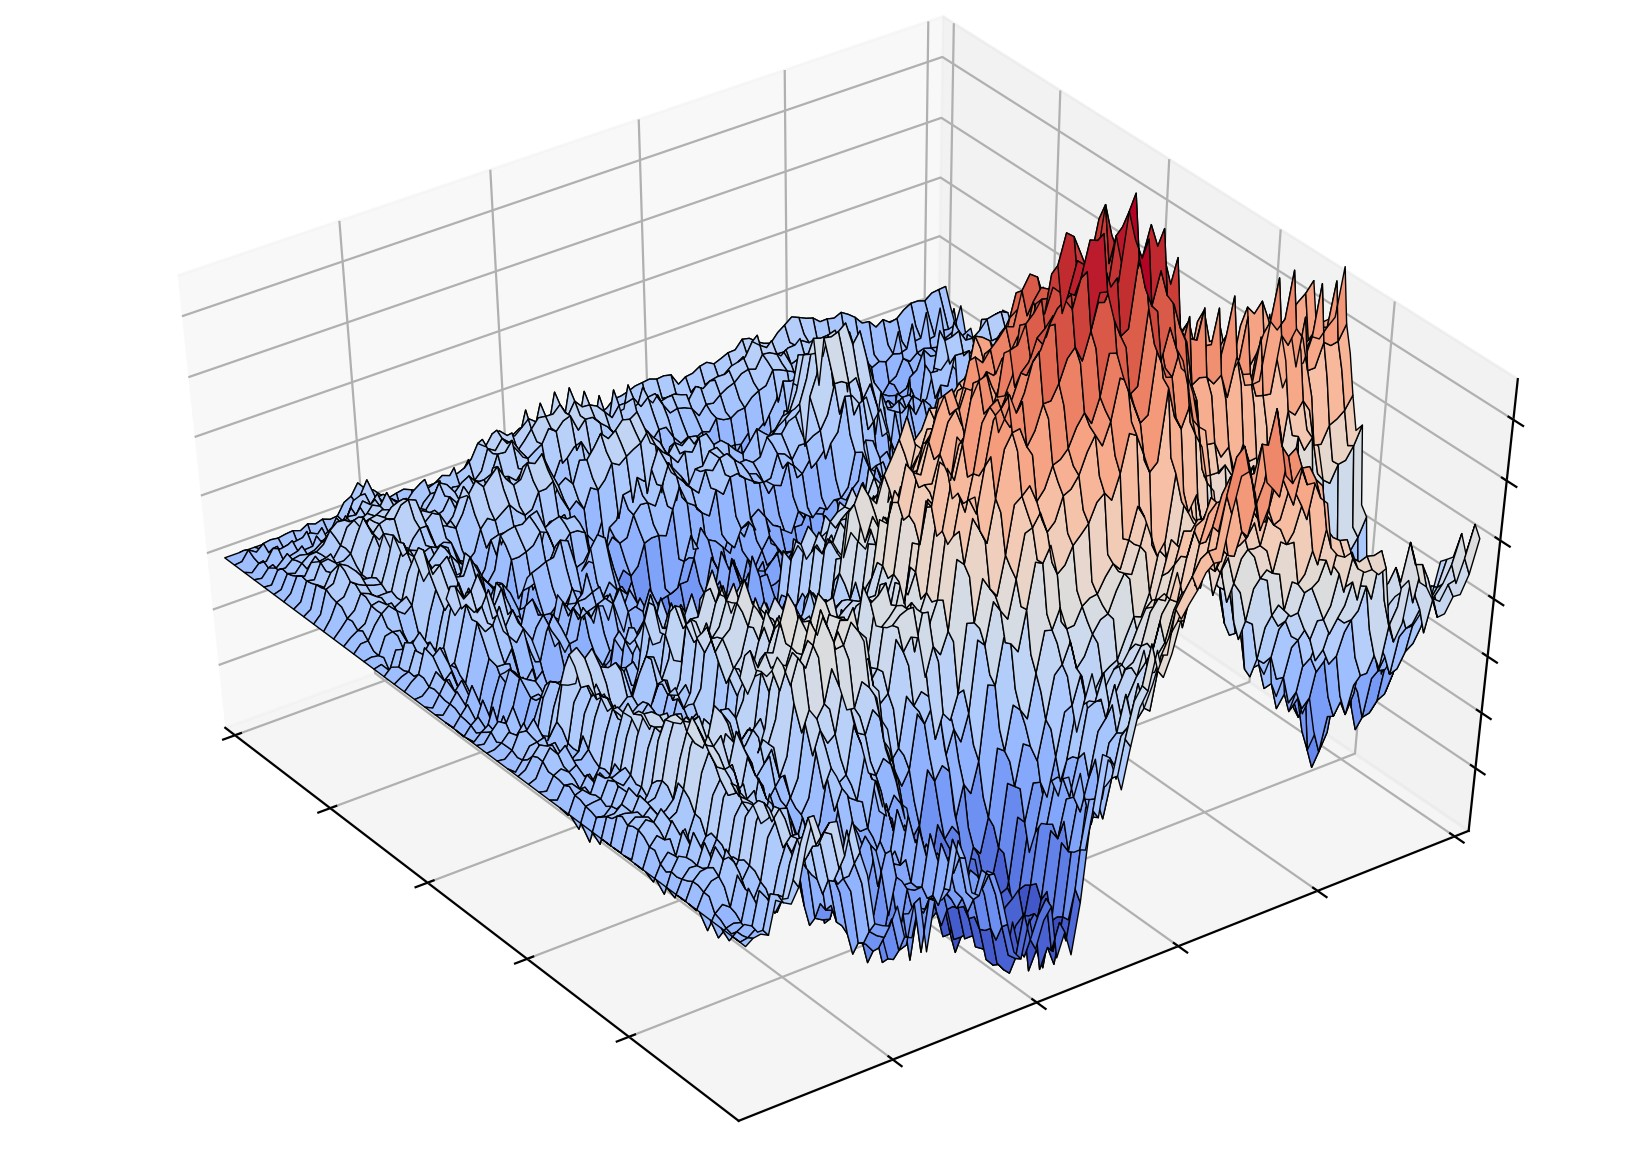
\includegraphics[scale=0.25]{browniansheet.png}
    \caption{Visualization of Brownian sheet}
\end{figure}

\subsection{Stochastic Heat Equation}
\subsection{Stochastic Wave Equation} Stochastic wave equation is helpful to model wave propagation in the media that exhibit some random variations. The inhomogeneous stochastic wave equation driven by a white noise is the following 
\begin{align}
    \left\{\begin{aligned}
        &\frac{\partial^2 v}{\partial t^2 } (x,t)= \frac{\partial^2 v}{\partial x^2} (x,t) + W(dx,dt)\\
       &v(x,0) = \frac{\partial v}{\partial t} (x,0) = 0
    \end{aligned}\right.
\end{align}

\subsection{Propagation of Singularities}
Recall the property of law of iterated logarithm of Brownian Motion, and its modulus of continuity, we further extend the result to Brownian Sheet and the solution to some specific SPDEs.

\newpage
\section{Random Field}
The stochastic processes we have discussed before are defined over a 1-dimensional time space. Here, random field generalizes the idea to a topological space $T$. The formal definition of random field is \\


    Consider a complete probability space $(\Omega, \mathcal{F},\mb{P})$, and a topological space $T$. The measurable function $f:\Omega \rightarrow \mf{R}^T (\text{or} \ \mathcal{C}(T,\mf{R}),\  \text{all real-valued functions on $T$})$ is said to be a random field. If $f$ takes value in d-dimensional space $\mf{R}^d$, we call it a vector valued random field, or $(N,d)$-random field. Also, if $\mf{R}^d$ is replaced by $\mb{Z}^d$, that is, $\{X_{\mf{i}}: \mf{i} \in \mb{Z}^d\}$ is a discrete random field. The discrete random field has been long studied in random models such as bond percolation and Ising model, which will be discussed later. 

\subsection{General Gaussian process}
The generalization of standard Brownian Motion is the $(N,\alpha,d)$ Gaussian Process. In Kahane J. P. (1985) \textit{Some Random Series of Functions}, it is defined as the process $X(t)$ from $\mathbb{R}^N$ to $\mf{R}^d$ such that $$\mb{E}\left[|X(t)-X(s)|^2\right] = d|t-s|^{2\alpha}.$$
Under this defintion, standard BM is the special case of $(1,d,\frac{1}{2})$-Gaussian Process, and the fractional Brownian Motion is $(1,d,\alpha)$-Gaussian Process with Hurst index $\alpha$. More generally, if $N > 1$, the process $X(t) = \left(X_1(t),\cdots,X_d(t)\right)$ where $t\in \mf{R}^n$ denotes a $(N,d)$-Gaussian Random Field. The theories in Markov process and martingales failed in studying Gaussian Random Field as the result of local dependence. However, there are some interesting properties of Gaussian Random Field, such as local nondeterminism (LND) and intermittency in SPDE, which will be discussed later. 

We continue to prove the existence of the $(N,\alpha,d)$-Gaussian process.

\subsection{Gaussian Free Field}
In this section, we will introduce the concept of discrete Gaussian Free field defined on lattice $D \subset \mb{Z}^d$ and its properties. There are two equivalent definitions of discrete GFF, it can be defined via either density function or Covariance function. Let's start with the discrete Laplacian operator  



\subsection{Hausdorff Measure}
The Hausdorff measure is a type of outer measure, and a generalization of the traditional notions of area and volume to non-integer dimensions.\\

\begin{definition}[Hausdorff measure]
    Let (X,d) be a metric space, and $|E|$ denote the diameter of set $E\subseteq X$. For every $d,\delta$, define $$\mathcal{H}_\delta^d (E)= \inf_{(F_i)} \left\{ \sum_{i=0}^\infty |F_i|^d : E\subseteq \bigcup_{i=1}^\infty F_i ;\ |F_i| < \delta  \right\},$$ and take the limit of $\delta$, the Hausdorff measure of $E$ is $$\mathcal{H}^d(E) = \lim_{\delta\downarrow 0} \mathcal{H}^d_\delta (E).$$ Moreover, the Hausdorff dimension is defined as $\displaystyle{\inf_{d}\left\{d\geq 0: \mathcal{H}^d(E) = 0\right\}}$
\end{definition}

To show that Hausdorff measure is indeed a well-defined measure, note that $\displaystyle{|E| = diam(E) := \sup_{x,y\in E}d(x,y)}$ is a pre-measure.

The following concepts extended the definition. \\

\begin{definition}[Exact Dimension Function]
    Let (X,d) be a metric space and $E \subseteq X$. Define the Hausdorff measure corresponding to the function $h:\mf{R}_+ \rightarrow \mf{R}_+$ as $$\mu _h(E) := \lim_{\delta \downarrow 0} \mu_{h,\delta}(E)$$ where 
    $$\mu_{h,\delta}(E) : = \inf_{(F_i)} \left\{ \sum_{i=0}^\infty h(|F_i|) : E\subseteq \bigcup_{i=1}^\infty F_i ;\ |F_i| < \delta  \right\}.$$ Then $h$ is called a dimension function (gauge function) for $E$ if $\mu_h(E) \in (0,\infty)$. Rogers(1998) has established some properties of a gauge function, i.e., $h$ should be monotonically increasing for $t\geq 0$, strictly positive for $t>0$, and continuous on the right for all $t\geq 0$. We refers to Rogers's book \cite{Rogers} for more information.

    So far, we have introduced some properties of Hausdorff measure, we continue to apply Hausdorff measure to study the sample path of Brownian Motion and Gaussian Process.
\end{definition}

\subsection{Spectral Analysis}
We first introduce some spectral properties of Gaussian random process and then discuss the general random field. As mentioned, the metric space $\left(\mf{R}^N,d\right)$, with $d(s,t) = |t-s|^\alpha$
In this section, we will introduce the basics of stochastic calculus


\newpage
\section{Diffusion Process}
\begin{quotation}
    \textit{The major objection to the study of diffusion theory by the method just described is that the hard machinery used comes from the theory of partial differential equations and the probabilistic input is relatively small. A more probabilistically satisfactory approach was suggested by Levy and carried out by Ito [1951]. The idea here is to return to the intuitive picture of $x(t+h) -x(t)$, for small $h>0$, looking like the Gaussian independent increment process with drift b(t,x(t)) and covariance a(t,x(t)).}\\
    \begin{flushright}------ Stroock, D. W., \& Varadhan, S. S. (1997)\end{flushright}
\end{quotation}

\newpage
\section{Random Graph}
This section is independent to the previous ones to some extent. The models presented here have a discrete flavour instead. We will discuss some probabilistic models such as bond percolation, Ising model and so on. We first introduce some interesting random models. The first two are examples of random cluster model.

\subsection{Ising model}
We first defines some terminologies. In the lattice model $\mb{Z}^d$, the hypercube can be defined as 
$$\Lambda := \left\{\mathbf{i}\in \mb{Z}^d : |\mathbf{i}|_{\infty} < k\right\}\quad \text{for some $k\in \mb{N}$},$$

we say $\omega = \left\{\omega_{\mf{i}} : \mf{i}\in \Lambda \right\}$ is a configuration on $\Lambda$, when $\omega_{\mf{i}}$, denoting the magnetic spin at site $\mf{i}$, takes values in the set $\{-1,+1\}$ for each $\mf{i}\in \Lambda$. We can derive a probability measure with a fixed configuration $\tilde{\omega}$. The energy function (Hamiltonian) is given by
$$H_{\Lambda,h,\tilde{\omega}} (\omega) = -J\left(\sum_{\mf{i,j}\in \Lambda, |\mf{i} - \mf{j}|_{1} = 1} \omega_{\mf{i}}\omega_{\mf{j}}+ \sum_{\mf{i}\in \Lambda, \mf{j}\notin \Lambda,|\mf{i} - \mf{j}|_{1} = 1} \omega_{\mf{i}}\tilde{\omega}_{\mf{j}}\right) - h \sum_{\mf{i}\in \Lambda} \omega_{\mf{i}}.$$

If the inverse temperature $\beta$ is fixed, the finite volume Ising probability measure on $\Lambda$ is defined as 
$$\mu_{\Lambda,\beta,h,\tilde{\omega}}(\omega) = \frac{\exp\left(-\beta H_{\Lambda,h,\tilde{\omega}}\right)}{Z_{\Lambda,\beta,h,\tilde{\omega}}}$$
where $Z_{\Lambda,\beta,h,\tilde{\omega}}$ is the normalizing constant.

Here we add some basic definitions from graph theory. A \textit{spanning subgraph} is a subgraph that contains all vertices of the original graph.

A nontrivial connected graph is $G$ called \textit{even} if for each vertex $v\in \mathcal{V}(G)$, there is a unique vertex $\bar{v} \in \mathcal{V}(G)$ such that $d(v,\bar{v}) = diam(G)$. In particular, an even graph $G$ is called \textit{symmetric} if $d(u,v) + d(u,\bar{v}) = diam(G)$ for all $u,v\in \mathcal{V}(G)$. 

\subsection{Percolation}
Percolation is a famous random graph model. Here we introduce the bond percolation model on lattice $\mb{Z}^d$ for $d\geq 2$. Let $\mb{E}^d$ denote the collection of edges between the nearest neighbours $\mf{x,y},|\mf{x} - \mf{y}| = 1$. For a given $\theta \in [0,1]$, we declare each bond in $\mb{E}^d$ to be \xt{open} with probability $\theta$ and closed otherwise, independently of all other bonds. The configuration $\mf{g}$ takes values in $\{0,1\}^{\mb{E}^d}$.

Now, given a configuration $\mf{g}$ and a point $\mf{x}\in \mb{Z}^d$, the cluster of $\mf{x}$, denoted by $\mathcal{C}(\mf{x})$, is collection of points that connects to $\mf{x}$. $\mathcal{C}(\mf{x})$ has the same distribution for all $\mf{x}$ because of the independence. The well-known phase transition property states that there is a critical probability space, we define $\Omega = \mb{R}^{I}$ $\theta_c$, where  
$$\rho(\theta) := \mathbb{P}\left(|\mathcal{C}(\mf{0})| = \infty\right) \quad \text{and}\quad  \theta_c = \sup\{\theta : \rho(\theta) = 0\}.$$
There are different proofs of the existence of critical probability, the classic one was by self-avoiding walk and the Kolmogorov 0-1 law, furthermore, Hugo Duminil-Copin and Vincent Tassion proposed a proof of the sharpness of the phase transition.$\blacksquare $ 

Figure 1 and 2 are visualizations of bond percolation simulation and the clusters by python.
\begin{figure}
    \centering
    \begin{subfigure}[b]{0.31\textwidth}
        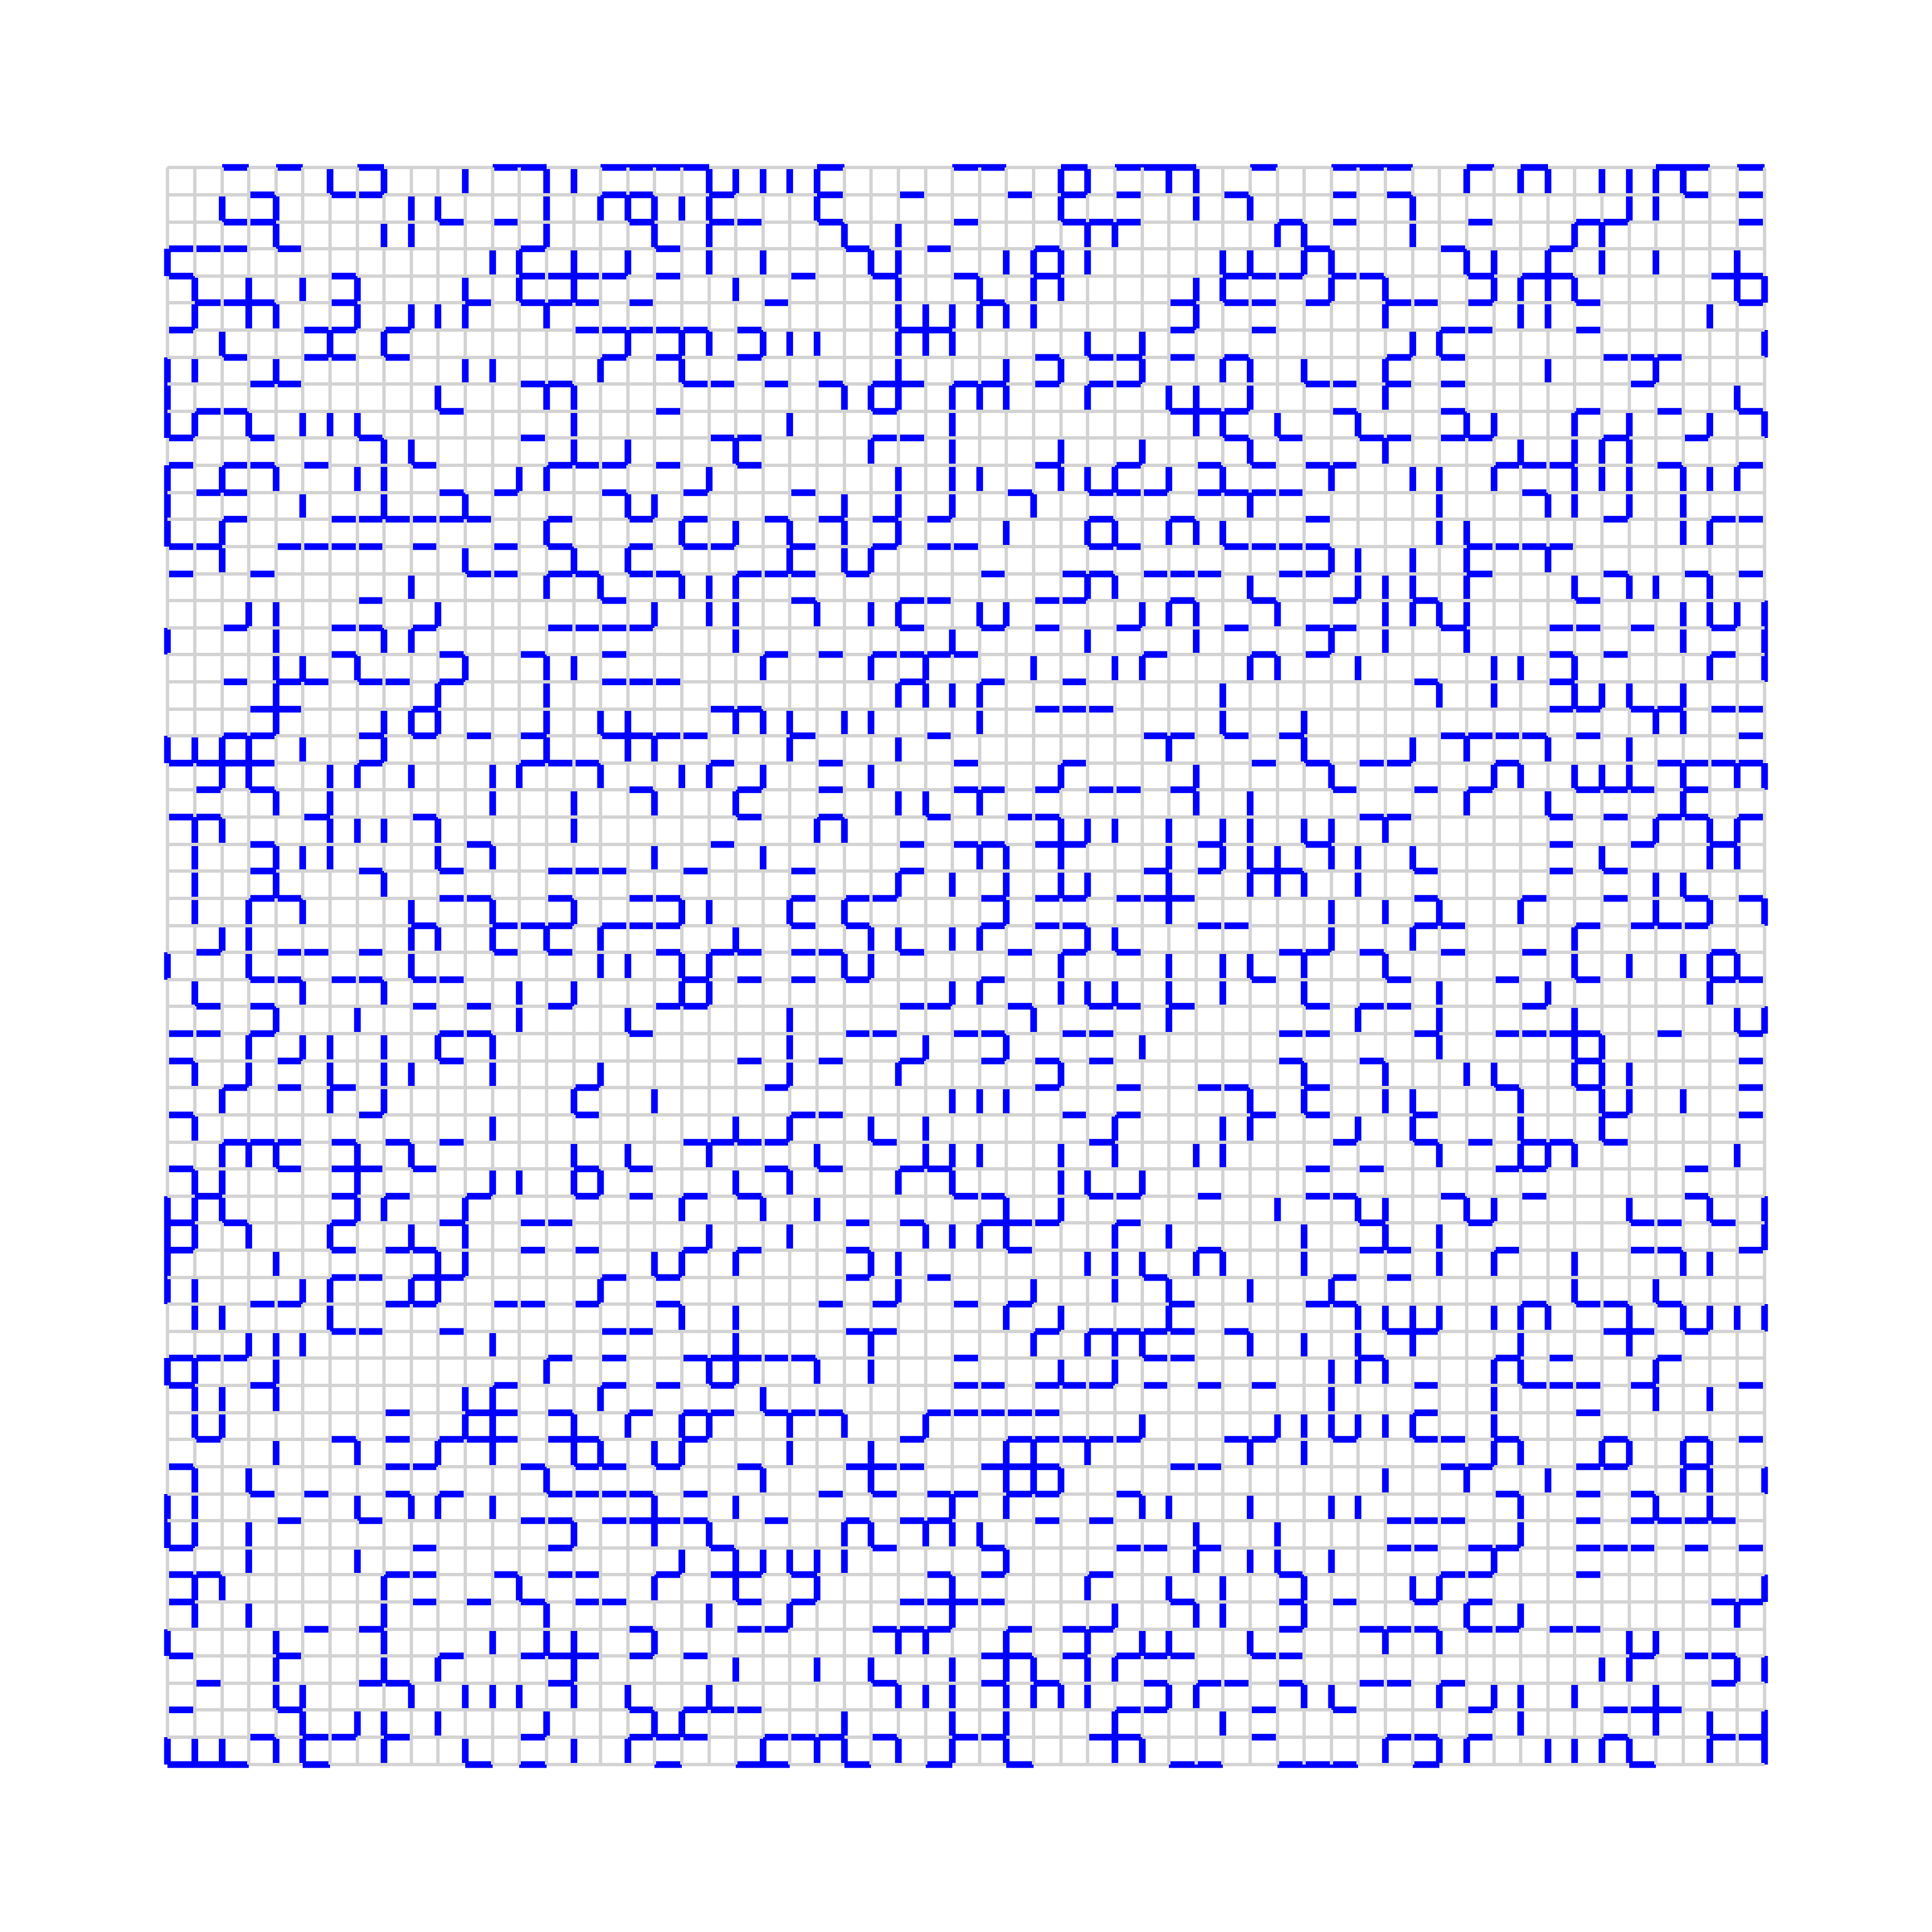
\includegraphics[width=\textwidth]{percolation_p0.3.png}
        \caption{$p=0.3$}
        \label{fig:gull}
    \end{subfigure}
    ~ %add desired spacing between images, e. g. ~, \quad, \qquad, \hfill etc. 
      %(or a blank line to force the subfigure onto a new line)
    \begin{subfigure}[b]{0.31\textwidth}
        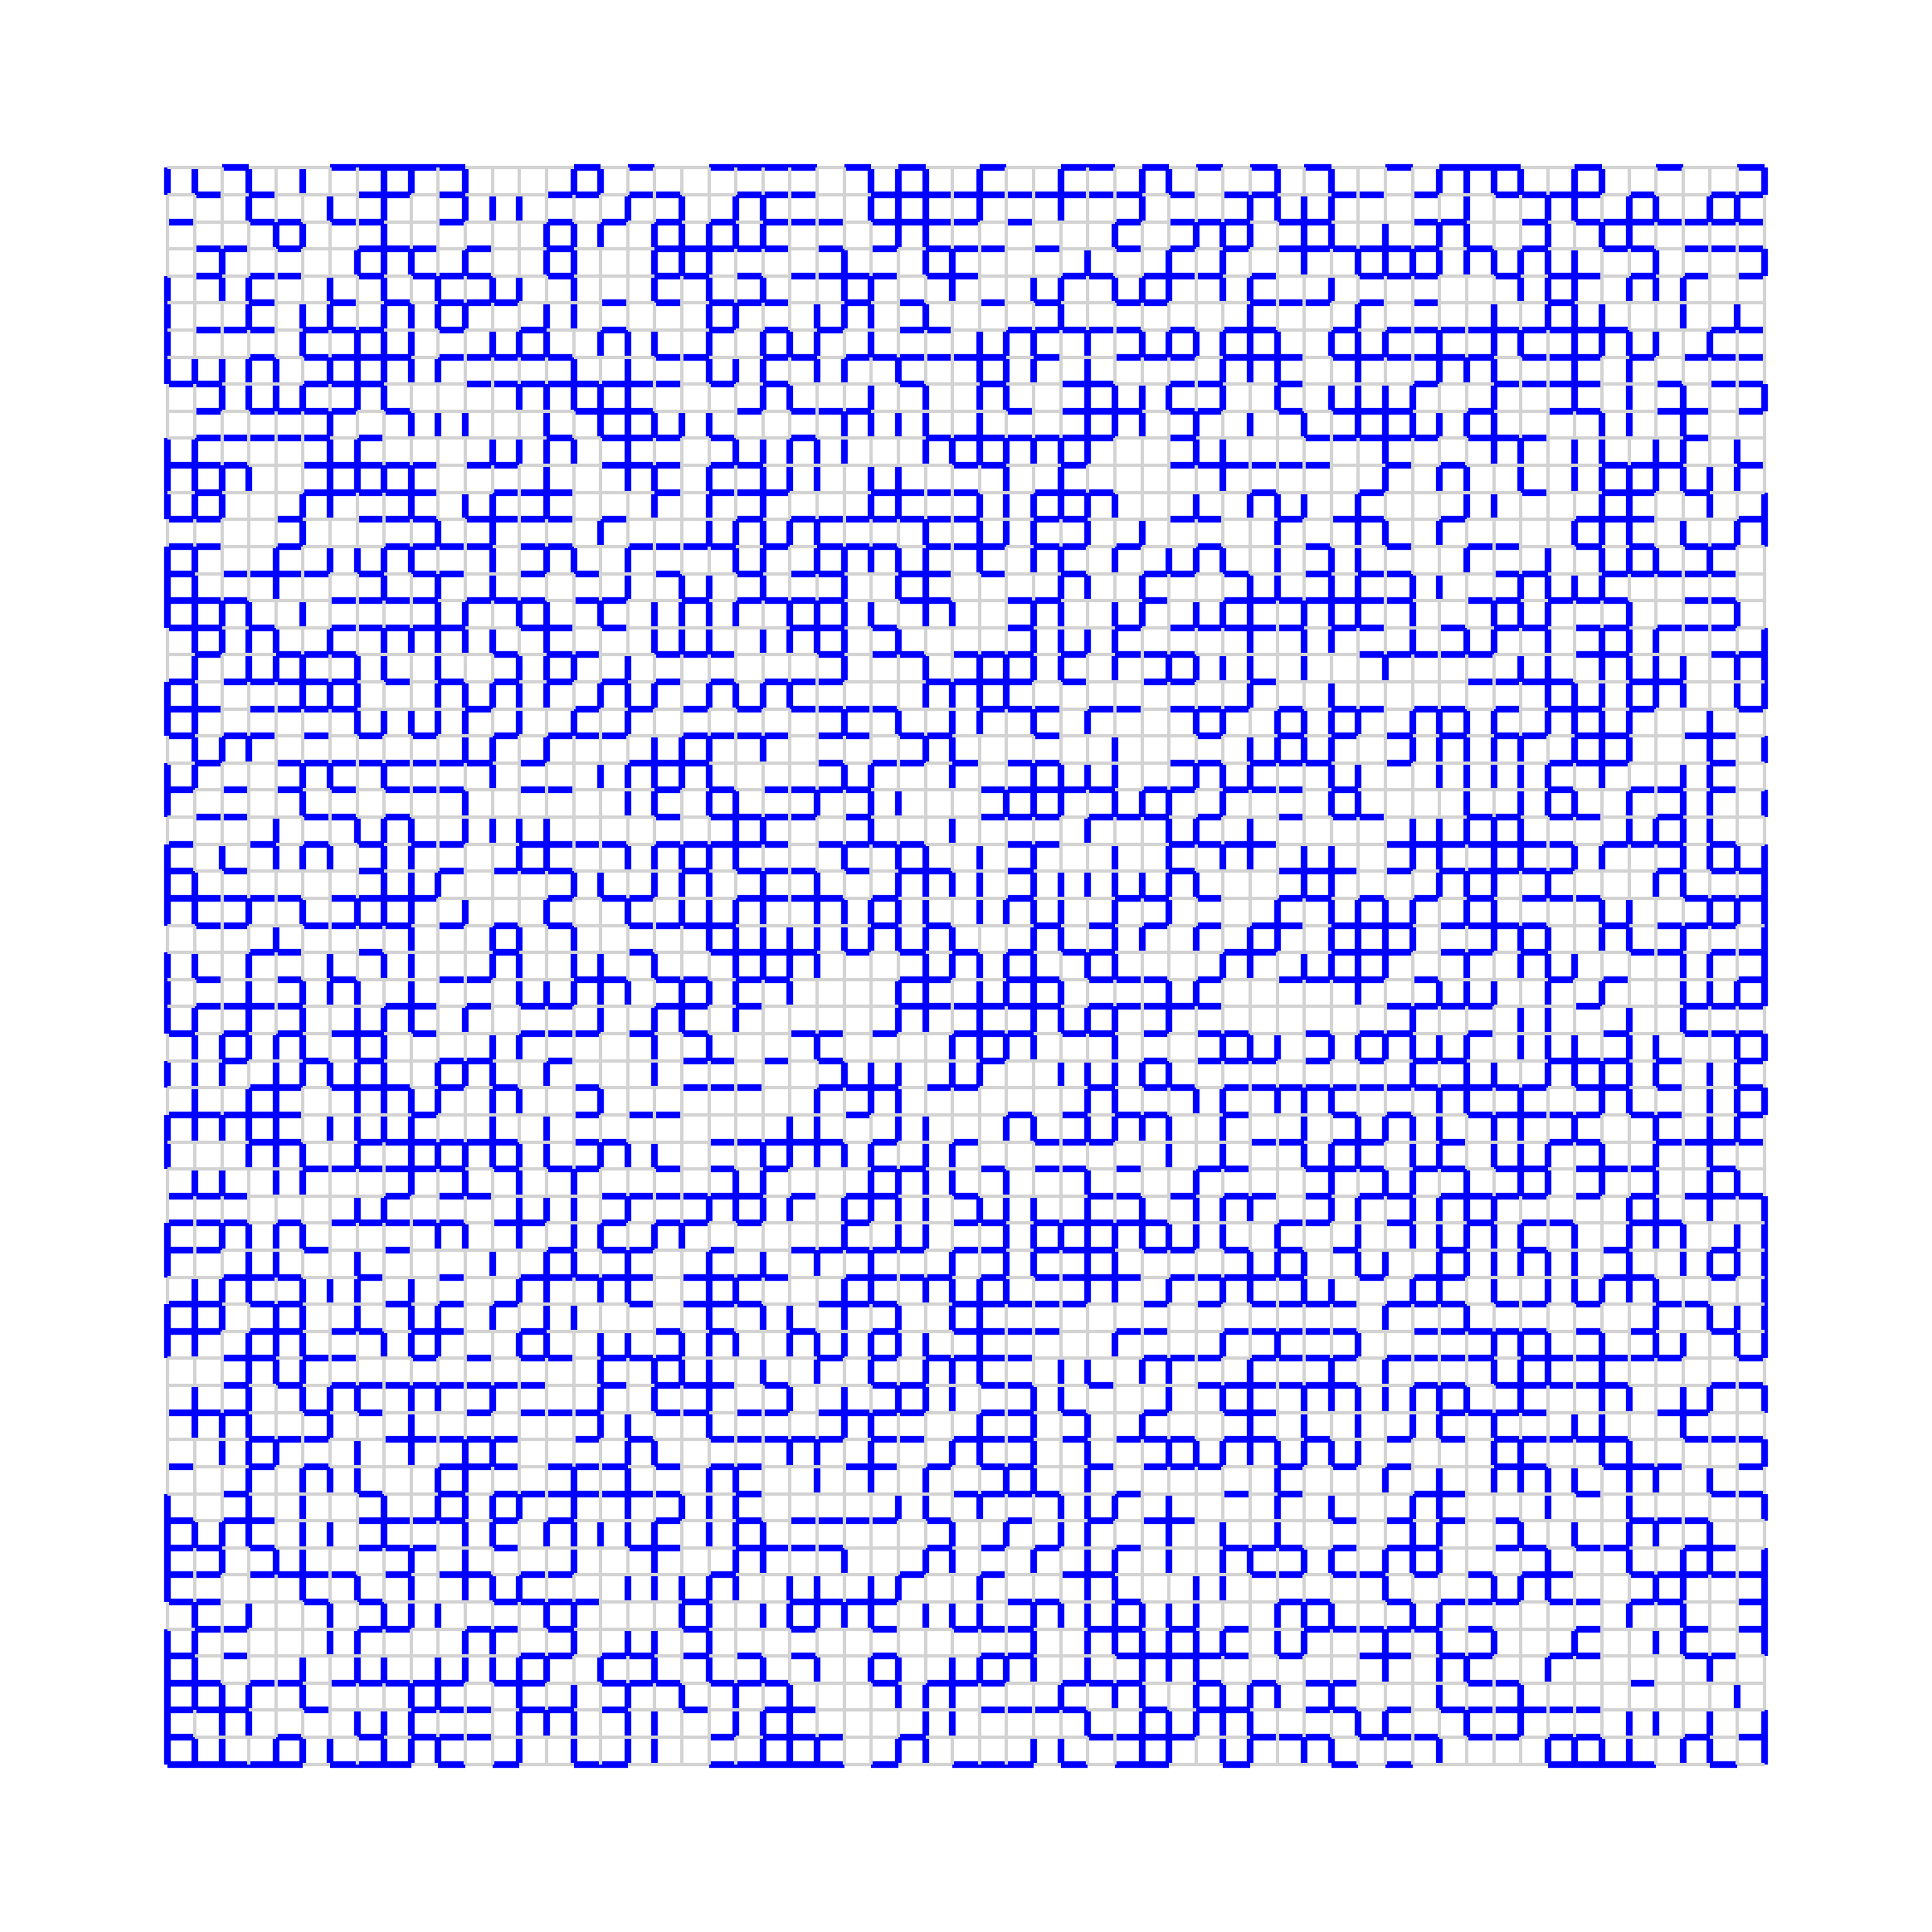
\includegraphics[width=\textwidth]{percolation_p0.5.png}
        \caption{$p=0.5$}
        \label{fig:tiger}
    \end{subfigure}
    ~ %add desired spacing between images, e. g. ~, \quad, \qquad, \hfill etc. 
    %(or a blank line to force the subfigure onto a new line)
    \begin{subfigure}[b]{0.31\textwidth}
        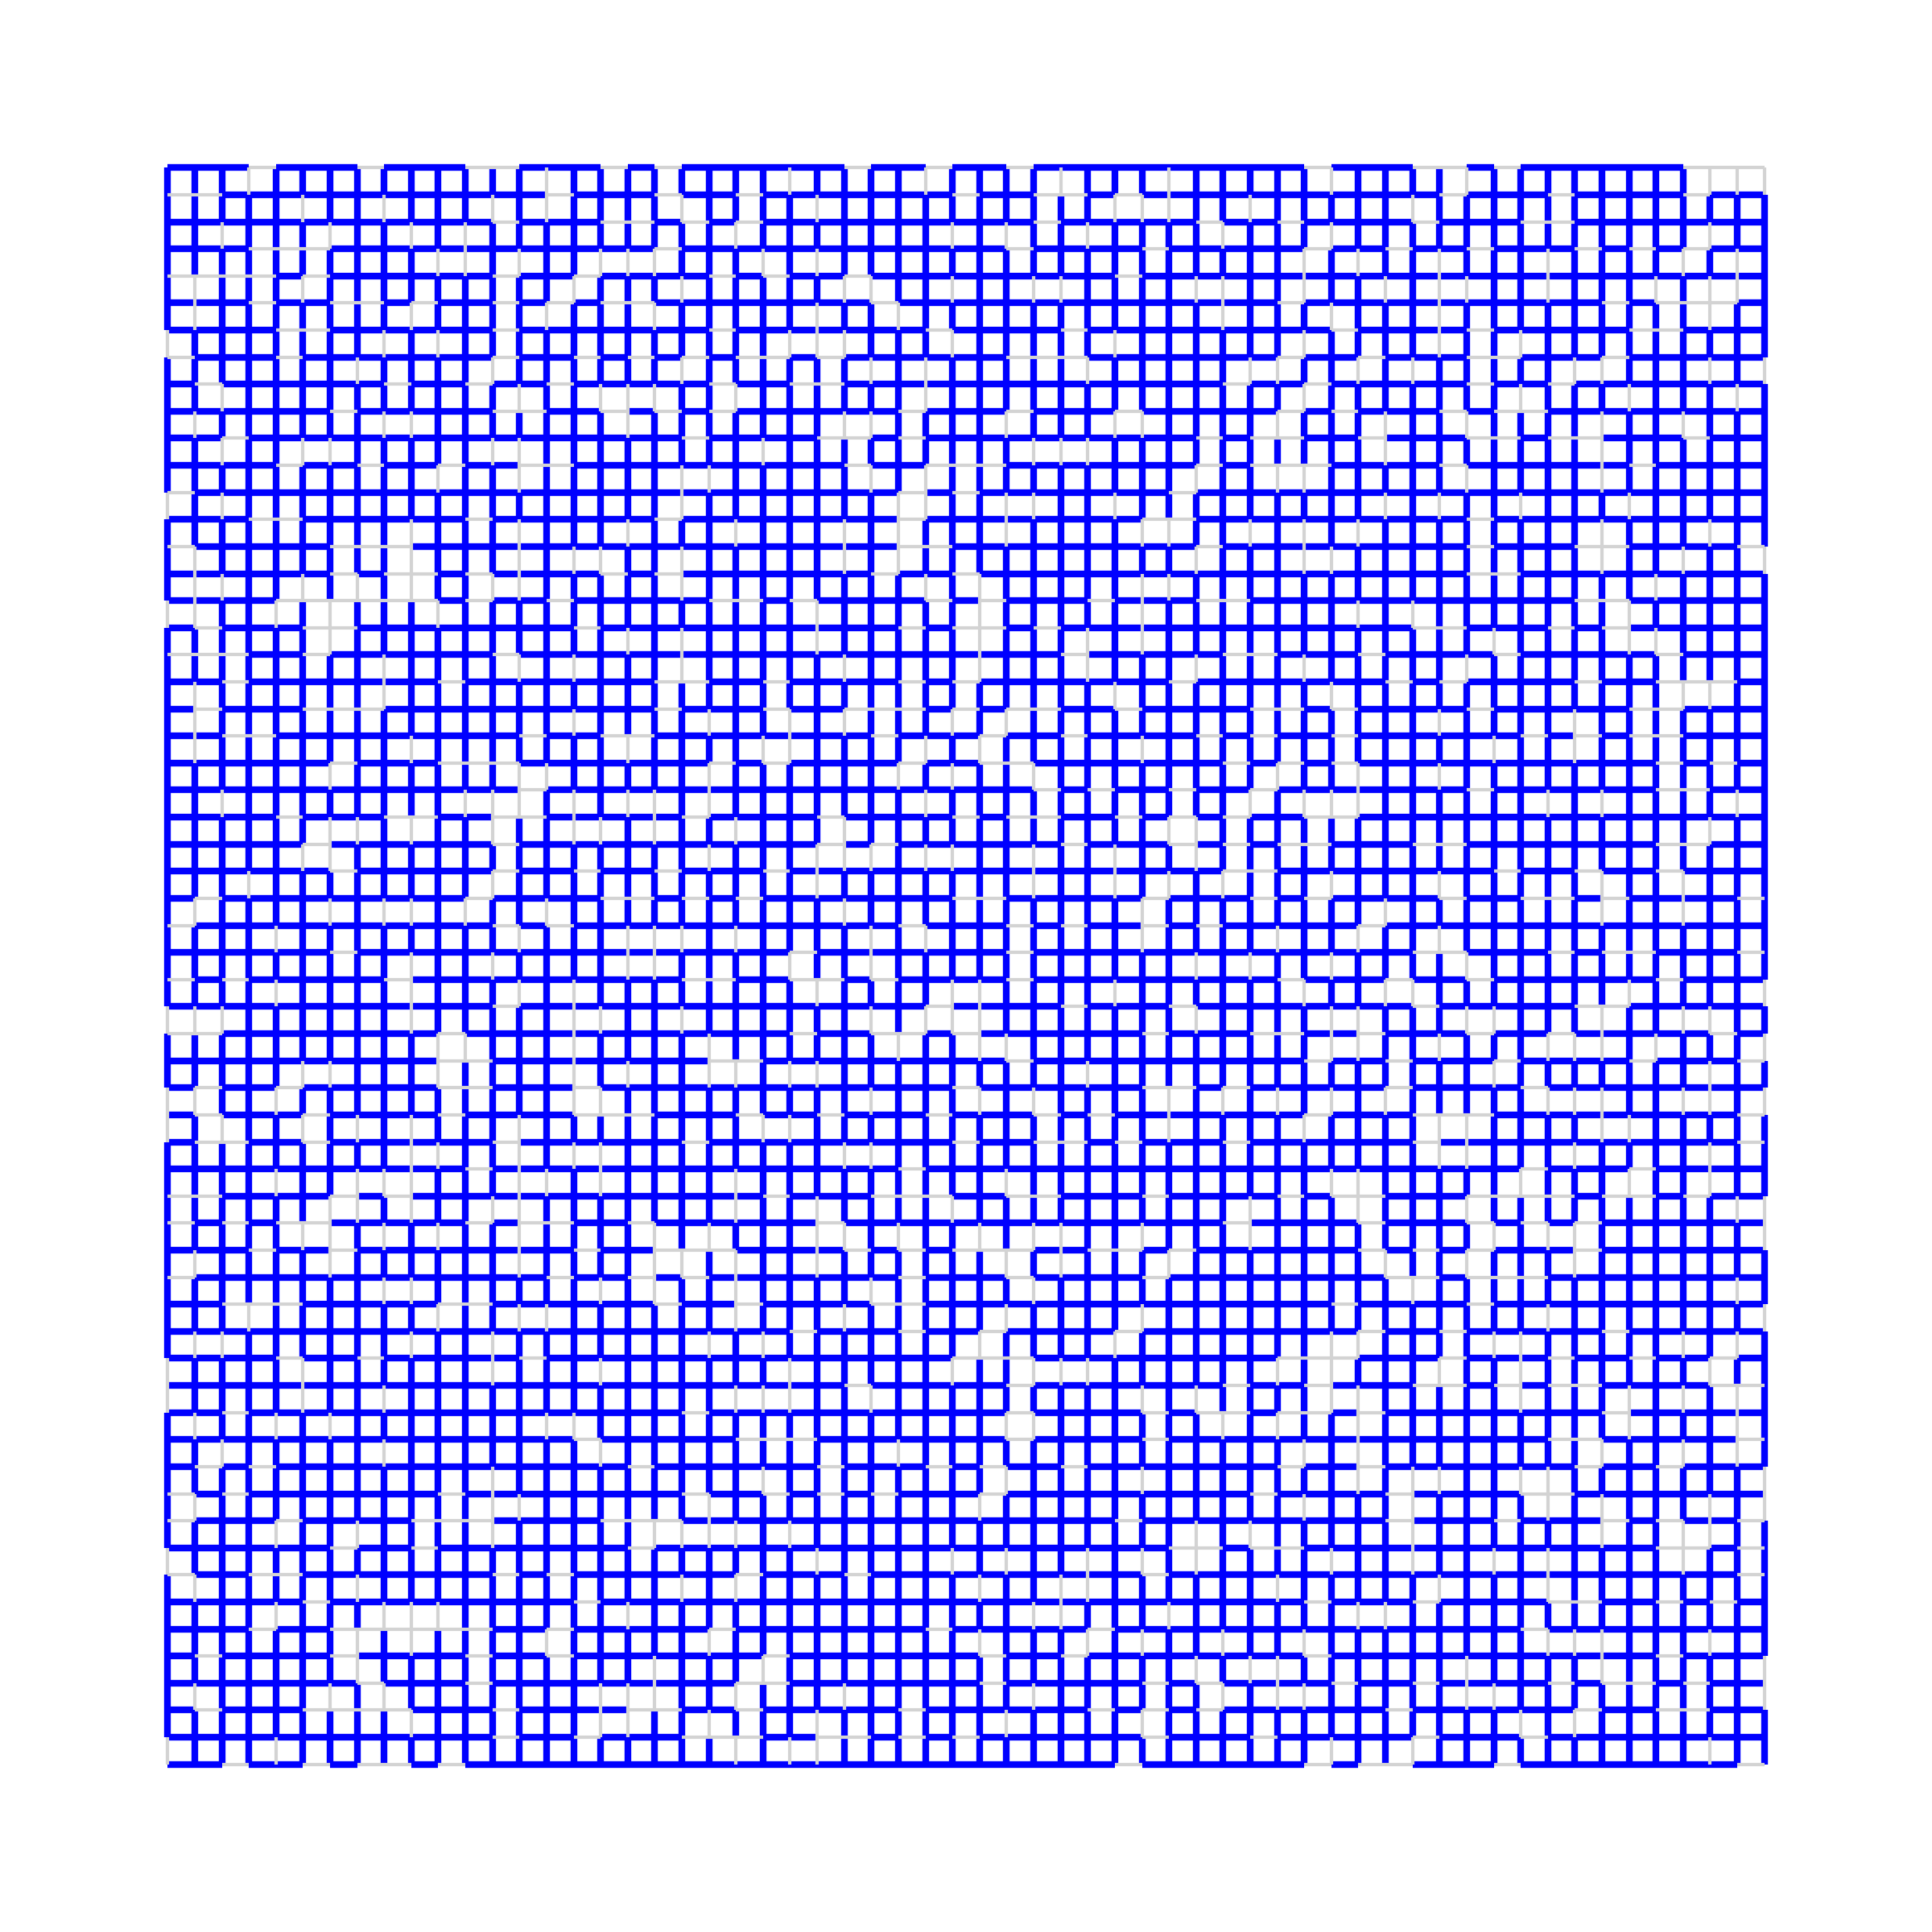
\includegraphics[width=\textwidth]{percolation_p0.8.png}
        \caption{$p=0.8$}
        \label{fig:mouse}
    \end{subfigure}
    \caption{Simulation of bond percolation}
\end{figure}

\begin{figure}
    \centering
    \begin{subfigure}[b]{0.29\textwidth}
        
\includegraphics[width=\textwidth]{cluster_p0.3.png}
        \caption{$p=0.3$}
    \end{subfigure}
    ~ %add desired spacing between images, e. g. ~, \quad, \qquad, \hfill etc. 
      %(or a blank line to force the subfigure onto a new line)
    \begin{subfigure}[b]{0.30\textwidth}
        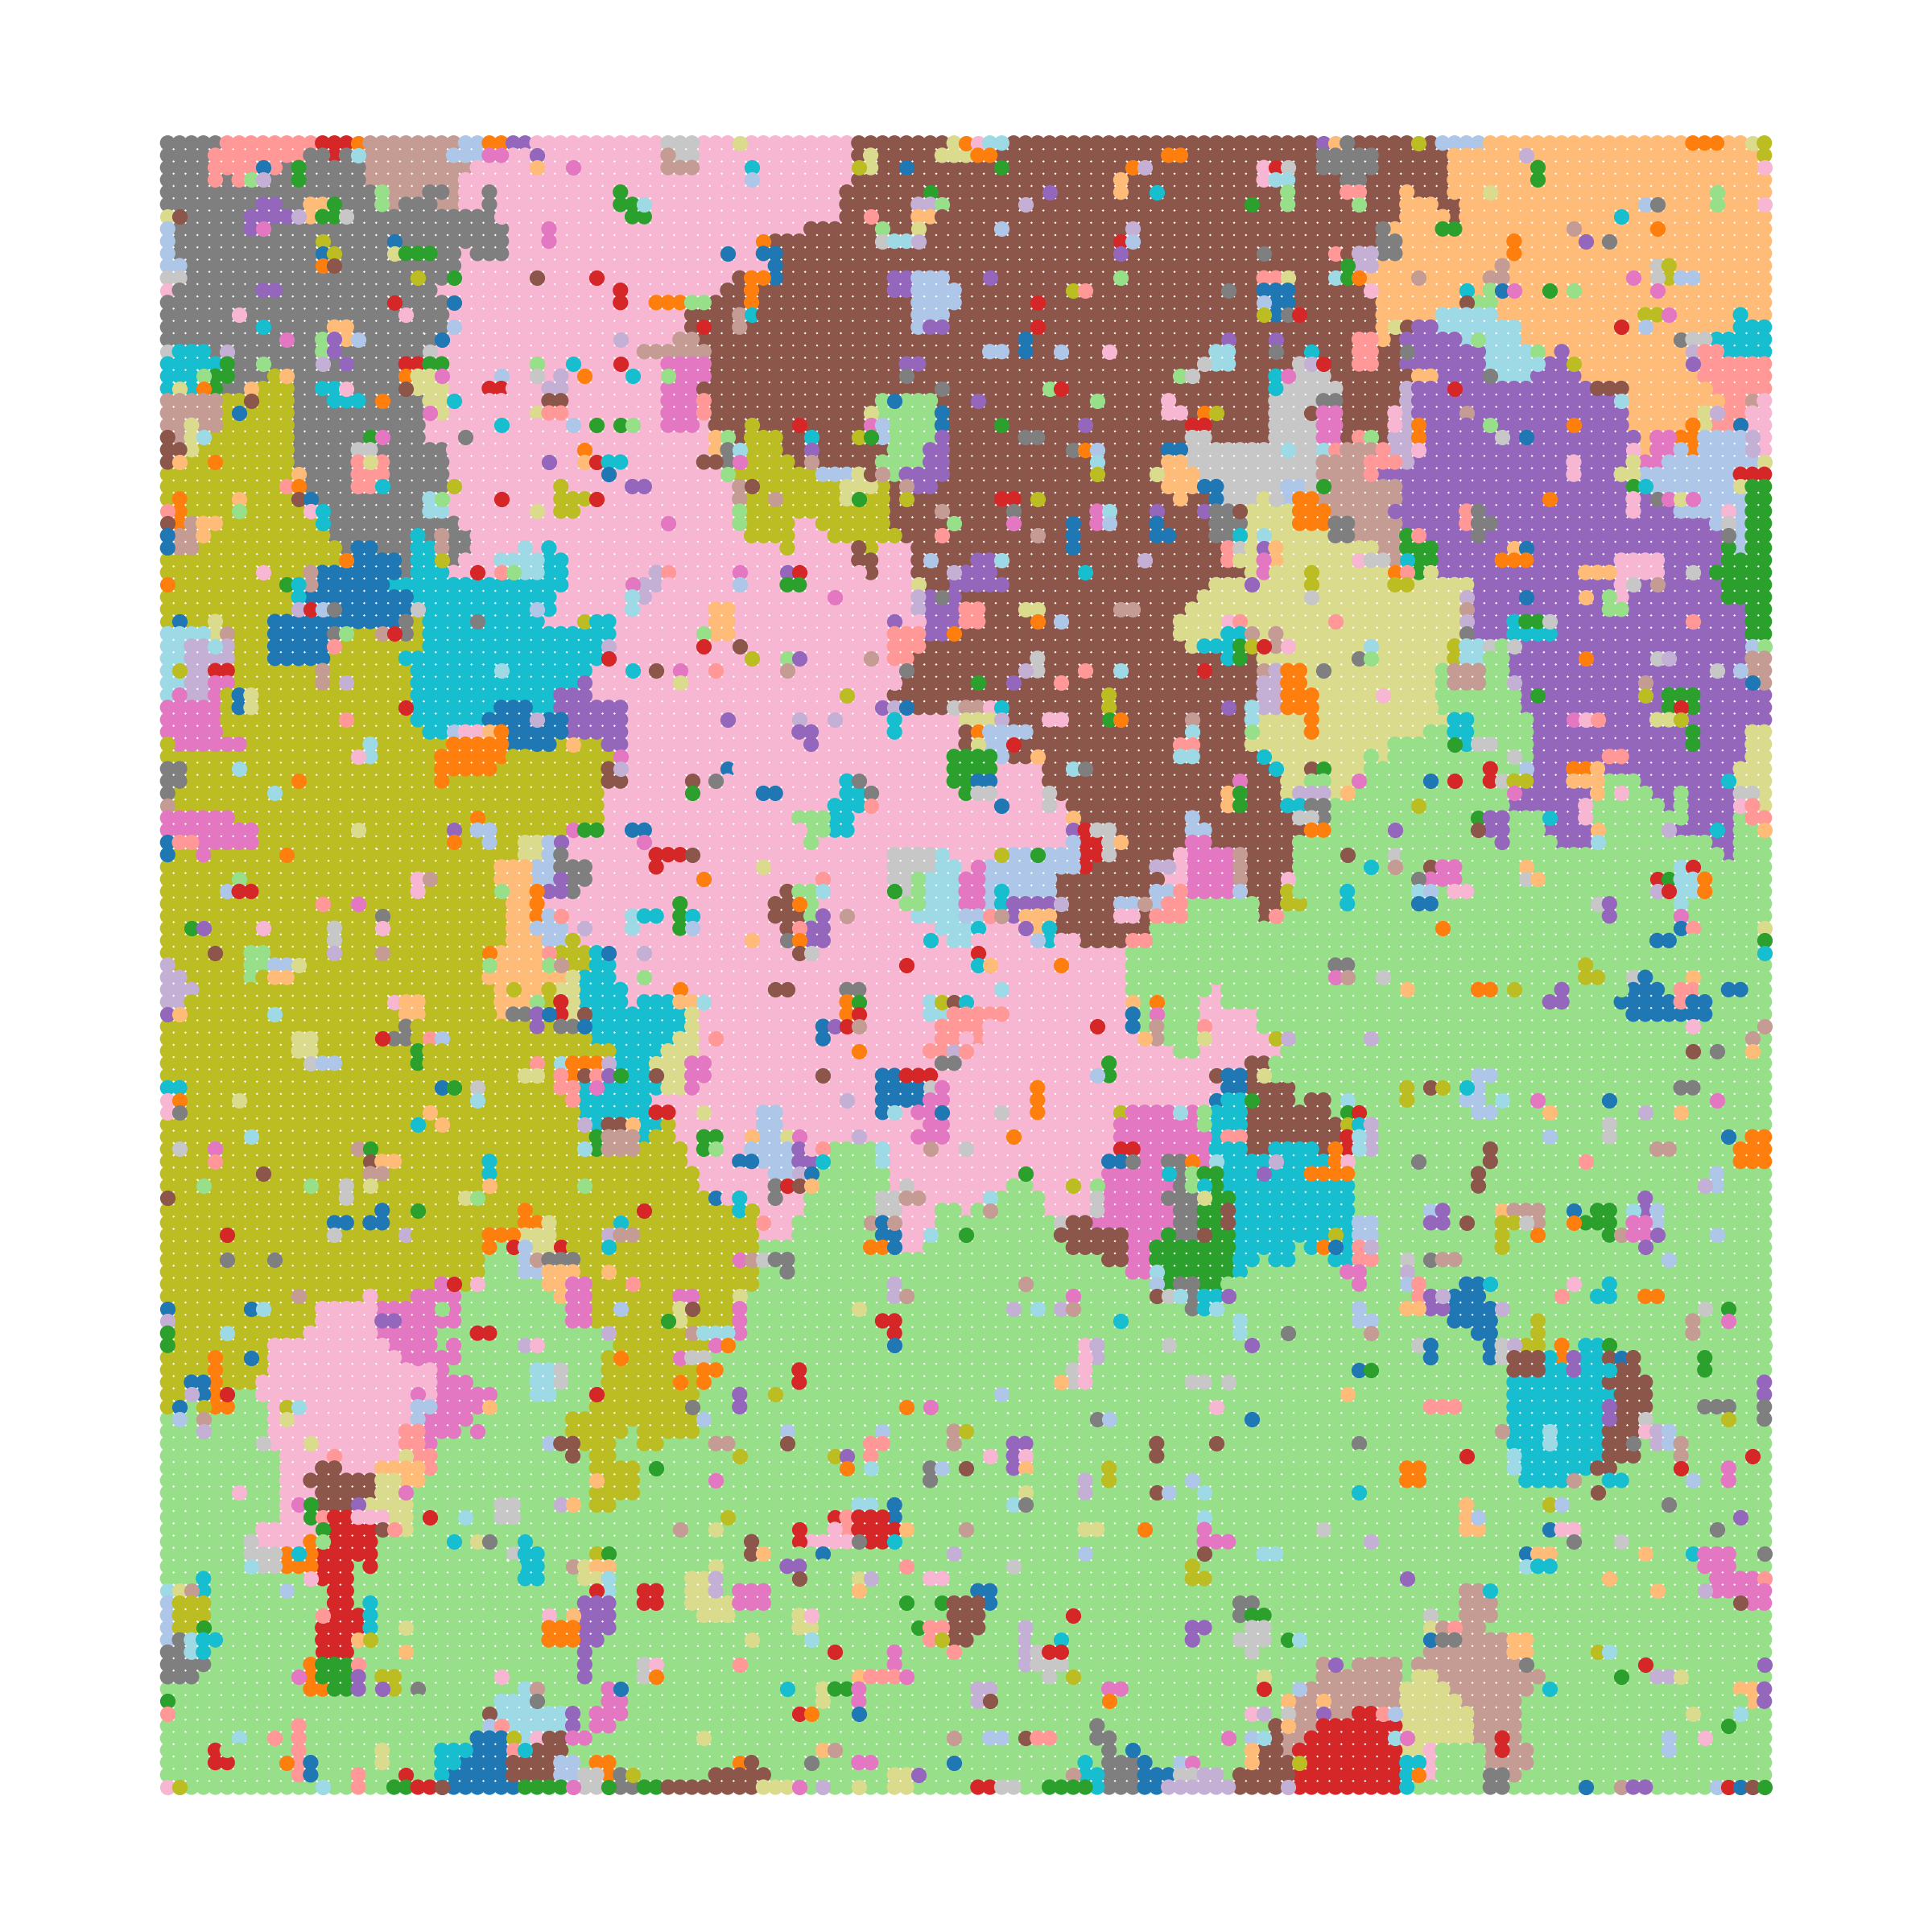
\includegraphics[width=\textwidth]{cluster_p0.5.png}
        \caption{$p=0.5$}
    \end{subfigure}
    ~ %add desired spacing between images, e. g. ~, \quad, \qquad, \hfill etc. 
    %(or a blank line to force the subfigure onto a new line)
    \begin{subfigure}[b]{0.30\textwidth}
        
\includegraphics[width=\textwidth]{cluster_p0.8.png}
        \caption{$p=0.8$}
    \end{subfigure}
    \caption{Simulation of clusters}
\end{figure}


We are interested in the supercritical case when $\theta > \theta_c$, the distribution of the total number of points in a finite block that belong to an infinite cluster, we define
$$\tau_{\mf{k}} = \sum_{\mf{x}\in B_{\mf{k}}^n} \mf{1}_{\{|\mathcal{C}(\mf{x})| = \infty\}}$$
where $B_{\mf{k}}^n = \{j\in \mb{Z}^d : k\leq j < k + n \mf{1}\}\subset \mb{Z}^d$.

\newpage
\section{Random Growth Model}
This section is the brief note of KPZ class, including different approaches to understand the universal scaling limit, the so-called $1:2:3$ KPZ scaling and other random models. The Kardar-Parisi-Zhang equation is, 
\begin{align}
    \partial_t h = -\lambda(\partial_x h)^2 + \nu \partial_x^2 h + \sqrt{D} \xi
\end{align}
where $\xi$ is the space-time white noise. $h:\mf{R}^d \times \mf{R}_+ \rightarrow \mf{R}$ can be understood as the height function of random growth model. We introduce the physical interpretation of KPZ equation by referring to \cite{Intro KPZ}. Consider the height function $h(x,t)$, there are three contributions to the random height function in the general form:
$$\partial_t h  = -\lambda F(\partial_xh) + \nu \partial^2_x h +\sqrt{D}\xi$$
\begin{enumerate}
    \item The diffusion term $\partial_x^2 h $ with diffusivity/viscosity $\nu$.
    \item The random forcing term $\xi$, which is commonly assumed to be a space-time white noise independent at different position and times. The Gaussian white noise has the correlation function: 
    $$R\left((t,x),(s,y)\right) = \mb{E}\left[\xi(x,t)\xi(y,s)\right] = \delta(t-s)\delta(x-y)$$
    Also, $\sqrt{D}$ represents the strength of noise.
    \item The first term is the deterministic part of the growth, it is assumed to be a symmetric function of the slope. The quadratic term $\partial_x^2h$ is a common choice.
\end{enumerate} 

The KPZ equation relates to other stochastic partial equations through some transformations. First, the stochastic Burgers equation
$$\partial_t u = -\lambda(\partial_x u^2) + \nu \partial_x^2 u + \sqrt{D}\partial_x \xi$$
and the stochastic heat eqation 
$$\partial_t u = \partial_x^2 u +\xi$$

\newpage 
\section{Random Matrix Theory and Free Probability}

\newpage
\section{Stein's Method}

We begin with a brief introduction on different probabilistic metrics. Stein's method serves as a great tool to bound these probabilistic distances.

\subsection{The Stein-Chen Method for Poisson Approximation}
The following part refers to the lecture note of SC2 by Professor Reinert, University of Oxford.

We first introduce the metric of two probability distributions, the \textit{total variation distance}. Suppose $P,Q$ are two probability distributions supported on the same probability space $(\Omega,\mathcal{F},\mu)$
$$d_{TV}(P,Q) \defeq \sup_{A\subset \Omega} |P(A) - Q(A)| $$

Total variation distance is a well-known distributional distance. A famous example is the bound for binomial and poisson distribution. Let $P \sim Binomial(n,p), Q \sim Poi(np)$, then
$$d_{TV}(P,Q) \leq p.$$
More precisely, Prohorov(1953)showed that 
$$d_{TV}(P,Q) \leq p\left[(2\pi e)^{-\frac{1}{2}} + \mathcal{O}\left(1\wedge \left(np\right)^{-\frac{1}{2}} + p\right)\right].$$
In general, the probability metrics between two probability measures $\mu,\nu$ on $(\Omega,\mathcal{F},\mb{P})$ have the form 
$$d_{\mathcal{H}}(\mu,\nu) = \sup_{h\in \mathcal{H}}\left|\int_\Omega hd\mu - \int_\Omega hd\nu \right|$$
where $\mathcal{H}$ is a functional space of test functions. The well-known example of test functions and corresponding metrics are
\begin{enumerate}
    \item Take $\mathcal{H} = \{\mf{1}_{[\cdot \leq x]},x\in\mf{R}\}$, we obtain the \textit{Kolmogorov Metric}. By its definition, convergence in Kolmogorov metric implies the weak convergence of probability measure. $\blacksquare $
    \item Take $\mc{H} = \text{Lip(1)}$, we obtain the so-called \textit{1-Wasserstein distance}
\end{enumerate}

\subsubsection{Stein's Method for Poisson Approximation}
We introduce the Poisson characterization. \\

\begin{lemma}
    Suppose $\Lambda$ is a probability distribution supported on $\mathbb{N}_0$, then $\Lambda \sim Poi(\lambda)$ if and only if
    $$\mb{E}\left[\lambda g(\Lambda+1) - \Lambda g(\Lambda)\right] = 0$$
    for all bounded function $g:\mb{N}_0 \rightarrow \mf{R}$.
\end{lemma}
\begin{proof}
    
\end{proof}
We introduce indicator functions to connect the TV distances of two random variables. The Stein-Chen Equation is the following:
$$\lambda g(j+1) - jg(j) = \mf{1}(j\in A) - Poi(\lambda)(A)$$
where $A \subset \mb{N}_0$. \\
\begin{lemma}
    Stein-Chen Equation has the following unique solution $g$,
    $$g^{(A,\lambda)}(j+1) = \frac{j!}{\lambda^{j+1}}e^{\lambda}\sum_{k=0}^j e^{-\lambda}\frac{\lambda^k}{k!}\left[\mf{1}(k\in A) - Poi(\lambda)(A)\right]$$
\end{lemma}
\begin{proof}
    
\end{proof}

There are variant properties of the solution function $g(\cdot) = g^{(A,\lambda)}(\cdot)$. Let $$||g||\defeq \sup_{j}|g^{(A,\lambda)}(j)|;\quad \bigtriangleup  g \defeq \sup_{j} |g^{(A,\lambda)}(j+1) - g^{(A,\lambda)}(j)|.$$

\begin{lemma}
    The solution function to Stein-Chen equation has the properties:
    $$||g|| \leq \min(1,\lambda^{-\frac{1}{2}});\quad \bigtriangleup g \leq \lambda^{-1}(1-e^{-\lambda}) \leq \min(1,\lambda^{-1})$$
\end{lemma}

The Stein's method for Poisson approximation deals with the TV distance between any random variable $X$ and $Poi(\lambda)$. Consider sets $A\subset \mb{N}_0$, and Stein's equation induced by $A$
$$\lambda g(j+1) - jg(j) = \mf{1}(j\in A) - Poi(\lambda)(A).$$
For any random variable $X$ we have 
$$\lambda g(X+1) - Xg(X) = \mf{1}(X \in A) - Poi(\lambda)(A).$$
Take expectation $\mb{E}_X[\cdot]$ of both sides,
\begin{align*}
    d_{TV}(\mathcal{L}(X),Poi(\lambda)) &= \sup_{A\in \mb{N}_0} \left|\mb{E}\left[\mf{1}(X\in A) - Poi(\lambda)\right]\right|\\
    &= \sup_g \left|\mb{E}[\lambda g(X+1) - Xg(X)]\right|
\end{align*}

We can take a step further to estimate $r.h.s$ uniformly. Consider independent indicator functions $I_1,\cdots,I_n$, and $\displaystyle{X = \sum_{i}I_i};\  X_i := \sum_{j\neq i}I_j$ then we can write
$$I_ig(X) = I_i g(X_i + 1)$$
Let $p_i = \mb{P}\left(I_i = 1 | I_1, \cdots, I_{i-1}\right)$, then the total variation distance $d_{TV}\left(\mathcal{L}(X),Poi(\lambda)\right)$ equals

$$d_{TV}\left(\mathcal{L}(X),Poi(\lambda)\right) = \sup_{g} \sum_{i} p_i \mb{E}\left[g(X+1) - g(X_i +1)\right]$$

In Barbour and Eagleson (1983), there are some bounds for the $r.h.s$. 


\subsubsection{Stein's Method for Normal Approximation}
We can extend the Poisson approximation approach to continuous distributions with some other distributional distances. Similarly, we first introduce the characteristic equation of standard normal distribution. \\
\begin{lemma}
    Suppose $Z$ is a random variable, then $Z\sim \mathcal{N}(0,1)$ if and only if 
    $$\mb{E}\left[Zf(Z)\right] = \mb{E}\left[f'(Z)\right]$$
    for all continuous and piecewise continuously differentiable functions $f:\mf{R}\rightarrow \mf{R}$ with $\mb{E}|f'(Z)| <\infty$
\end{lemma}
\begin{proof}
    
\end{proof}
Recall that solving the Stein-Chen equation can be help of deriving bounds for total variaton distance. Similarly, the Stein's equaton (for $h$) is the following
$$f'(w) - wf(w) = h(w) - \mb{E}|h(Z)| $$
where $Z\sim \mathcal{N}(0,1).$

In Stein's equation, the solution $f_h(\cdot)$ is dependent of $h$. \\

\begin{lemma}
    The unique and bounded solution to Stein's equation $f'(w) - wf(w) = h(w) - \mb{E}|h(Z)|$ is given by 
    \begin{align*}
        f_h(w) = e^{\frac{w^2}{2}} \int_{-\infty}^w (h(x) - \mb{E}|h(Z)|) e^{-\frac{x^2}{2}} dx
    \end{align*}
\end{lemma}

The solution $f_h$ obtains boundness of its derivative. \\
\begin{lemma}
    For bounded $h$ and the solution $f_h(\cdot)$ to Stein's equation has the following properties
    \begin{align*}
        & ||f_h|| \leq \sqrt{\frac{\pi}{2}} ||h(\cdot) -\mb{E}h(Z) ||\\
        & ||f_h'|| \leq 2||h(\cdot) - \mb{E}h(Z)||
    \end{align*}
    Moreover, for continuous and piecewise continuously differentiable $h:\mf{R}\rightarrow \mf{R}$, $f_h$ satisfies 
    \begin{align*}
       & ||f_h|| \leq 2||h'|| ;\quad ||f'_h|| \leq \sqrt{\frac{2}{\pi}} ||h'||; \quad ||f''_h|| \leq 2||h'||
    \end{align*}
\end{lemma}

\subsubsection{Two Approaches to Construct Stein Operator}
In this subsection, we will introduce two different method to construct the Stein's operator. The first method is the density approach that derived from integration by part. The second method introduced by Barbour, is the generator approach that generalize the idea to Stochastic process. \\
\textbf{Density Approach} Let $p(x)$ be a probability distribution, then for any suitable $f$ that satisfies $\lim_{x\rightarrow \infty} f(x)p(x) = 0$ and $f(0)=0$, we have 
\begin{align}
    \mb{E}\left[f(x)\nabla_x \log p(x) + \nabla_x f(x)\right] = 0 
\end{align}
To prove the above equality, we apply integration by part. \begin{align*}
    \mb{E}\left[f(x)\nabla_x \log p(x) + \nabla_x f(x)\right]&=  \int_\Omega f(x) \frac{p'(x)}{p(x)} p(x)dx + \int_\Omega \nabla_x f(x) p(x) dx\\ 
    & = f(x)p(x)|_\Omega - \int_\Omega \nabla_x f(x)  p(x) dx +\int_\Omega \nabla_x f(x) p(x) dx\\
    & = 0
\end{align*}



\subsection{Malliavin-Stein's Method}





\newpage
\section{Brownian Map}
This section will introduce some beautiful results of Brownian map. Here comes an amazing graphical example of sphere brownian map. 
\begin{figure}
    \centering
    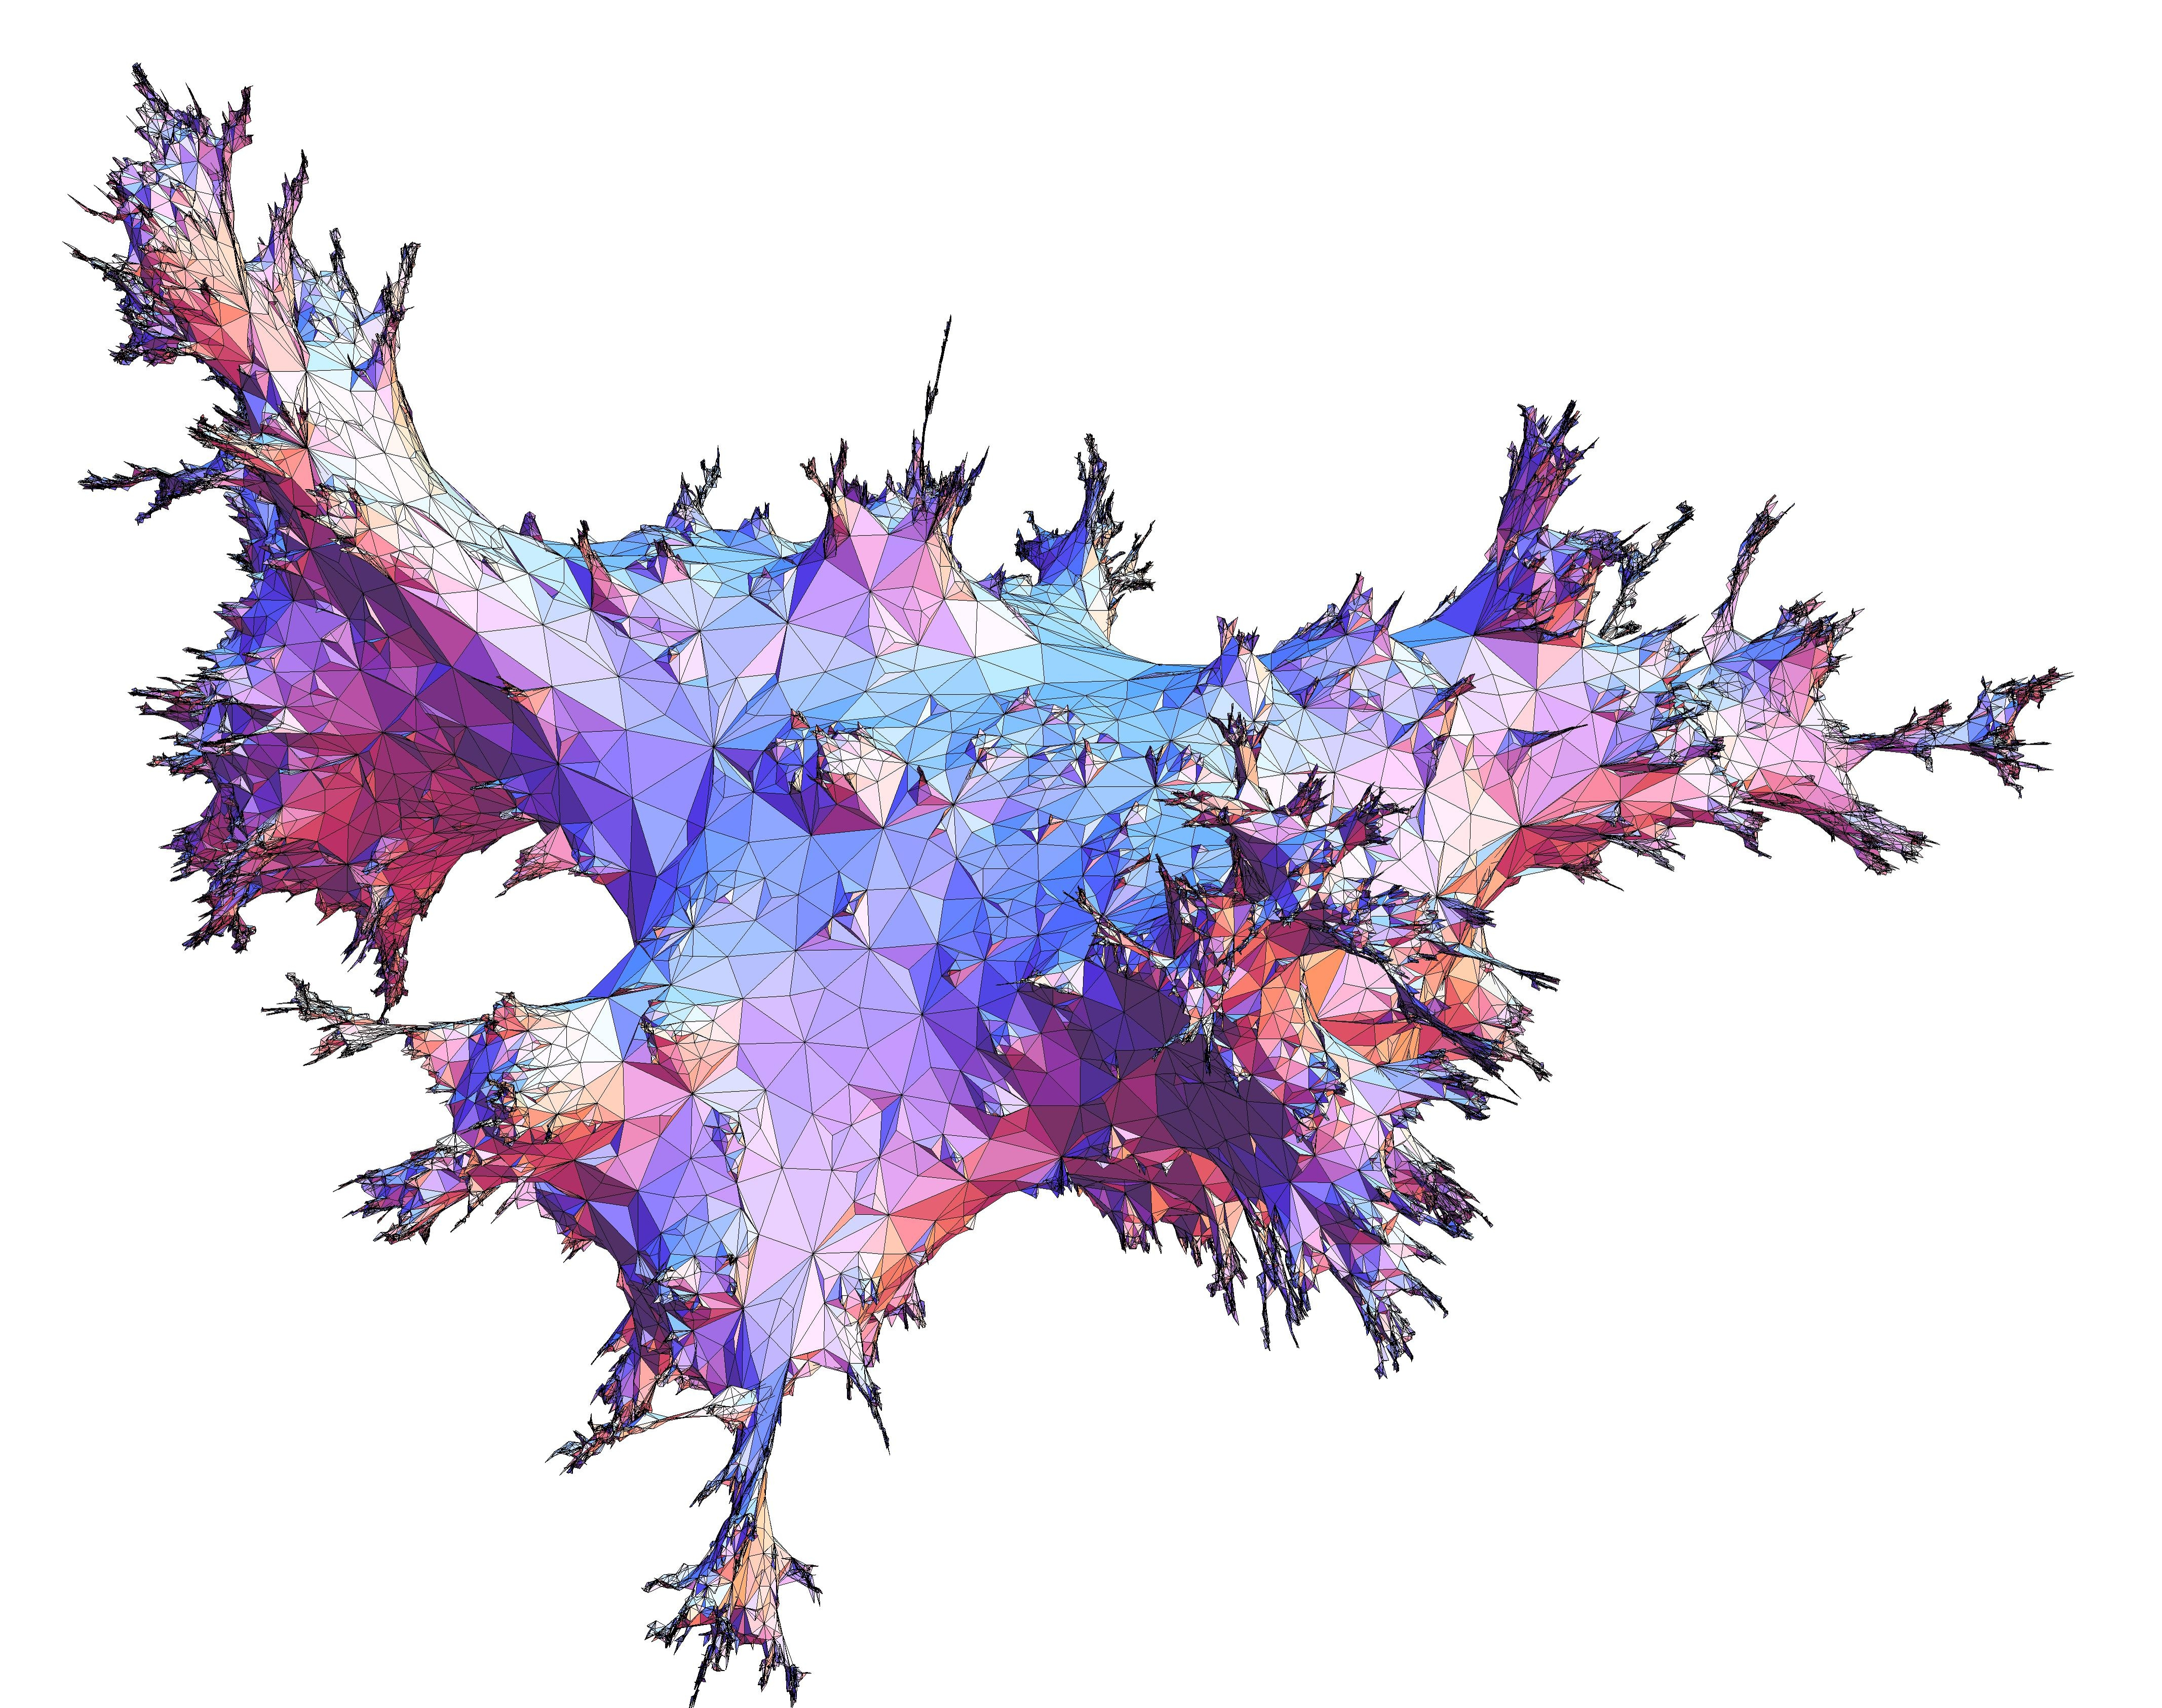
\includegraphics[scale=0.05]{Brownian map.png}
    \caption{Uniform triangualation}
\end{figure}



\begin{thebibliography}{999}
    \bibitem{Rogers}
    Rogers, C. A. (1998). Hausdorff measures. Cambridge University Press.
    
    \bibitem{Garrido-Ergodicity}
    Garrido-Atienza, M. J., \& Schmalfu\ss, B. (2011). Ergodicity of the infinite dimensional fractional Brownian motion. Journal of Dynamics and Differential Equations, 23(3), 671-681.

    \bibitem{Talagrand-hausdorfffbM}
    Talagrand, M. (1995). Hausdorff measure of trajectories of multiparameter fractional Brownian motion. The annals of Probability, 767-775.

    \bibitem{113}
    Karatzas, I., Shreve, S. E., Karatzas, I., \& Shreve, S. E. (1998). Brownian motion. Brownian motion and stochastic calculus, 47-127.

    \bibitem{Intro KPZ}
    Quastel, J. (2011). Introduction to KPZ. Current developments in mathematics, 2011(1).

    \bibitem{Varadhan-diffusion}
    Stroock, D. W., \& Varadhan, S. S. (1997). Multidimensional diffusion processes (Vol. 233). Springer Science \& Business Media.

    \bibitem{UCB-Dudley}
    Bartlett, P. (2013). Theoretical Statistics. Lecture 12.

    \bibitem{Orey&Taylor}
    Orey, S., \& Taylor, S. J. (1974). How often on a Brownian path does the law of iterated logarithm fail?. Proceedings of the London Mathematical Society, 3(1), 174-192.
    
\end{thebibliography}


\end{document}


